\documentclass[twoside]{book}

% Packages required by doxygen
\usepackage{fixltx2e}
\usepackage{calc}
\usepackage{doxygen}
\usepackage{graphicx}
\usepackage[utf8]{inputenc}
\usepackage{makeidx}
\usepackage{multicol}
\usepackage{multirow}
\PassOptionsToPackage{warn}{textcomp}
\usepackage{textcomp}
\usepackage[nointegrals]{wasysym}
\usepackage[table]{xcolor}

% Font selection
\usepackage[T1]{fontenc}
\usepackage{mathptmx}
\usepackage[scaled=.90]{helvet}
\usepackage{courier}
\usepackage{amssymb}
\usepackage{sectsty}
\renewcommand{\familydefault}{\sfdefault}
\allsectionsfont{%
  \fontseries{bc}\selectfont%
  \color{darkgray}%
}
\renewcommand{\DoxyLabelFont}{%
  \fontseries{bc}\selectfont%
  \color{darkgray}%
}
\newcommand{\+}{\discretionary{\mbox{\scriptsize$\hookleftarrow$}}{}{}}

% Page & text layout
\usepackage{geometry}
\geometry{%
  a4paper,%
  top=2.5cm,%
  bottom=2.5cm,%
  left=2.5cm,%
  right=2.5cm%
}
\tolerance=750
\hfuzz=15pt
\hbadness=750
\setlength{\emergencystretch}{15pt}
\setlength{\parindent}{0cm}
\setlength{\parskip}{0.2cm}
\makeatletter
\renewcommand{\paragraph}{%
  \@startsection{paragraph}{4}{0ex}{-1.0ex}{1.0ex}{%
    \normalfont\normalsize\bfseries\SS@parafont%
  }%
}
\renewcommand{\subparagraph}{%
  \@startsection{subparagraph}{5}{0ex}{-1.0ex}{1.0ex}{%
    \normalfont\normalsize\bfseries\SS@subparafont%
  }%
}
\makeatother

% Headers & footers
\usepackage{fancyhdr}
\pagestyle{fancyplain}
\fancyhead[LE]{\fancyplain{}{\bfseries\thepage}}
\fancyhead[CE]{\fancyplain{}{}}
\fancyhead[RE]{\fancyplain{}{\bfseries\leftmark}}
\fancyhead[LO]{\fancyplain{}{\bfseries\rightmark}}
\fancyhead[CO]{\fancyplain{}{}}
\fancyhead[RO]{\fancyplain{}{\bfseries\thepage}}
\fancyfoot[LE]{\fancyplain{}{}}
\fancyfoot[CE]{\fancyplain{}{}}
\fancyfoot[RE]{\fancyplain{}{\bfseries\scriptsize Generated on Sun Jan 29 2017 14\+:02\+:32 for Jackpot by Doxygen }}
\fancyfoot[LO]{\fancyplain{}{\bfseries\scriptsize Generated on Sun Jan 29 2017 14\+:02\+:32 for Jackpot by Doxygen }}
\fancyfoot[CO]{\fancyplain{}{}}
\fancyfoot[RO]{\fancyplain{}{}}
\renewcommand{\footrulewidth}{0.4pt}
\renewcommand{\chaptermark}[1]{%
  \markboth{#1}{}%
}
\renewcommand{\sectionmark}[1]{%
  \markright{\thesection\ #1}%
}

% Indices & bibliography
\usepackage{natbib}
\usepackage[titles]{tocloft}
\setcounter{tocdepth}{3}
\setcounter{secnumdepth}{5}
\makeindex

% Hyperlinks (required, but should be loaded last)
\usepackage{ifpdf}
\ifpdf
  \usepackage[pdftex,pagebackref=true]{hyperref}
\else
  \usepackage[ps2pdf,pagebackref=true]{hyperref}
\fi
\hypersetup{%
  colorlinks=true,%
  linkcolor=blue,%
  citecolor=blue,%
  unicode%
}

% Custom commands
\newcommand{\clearemptydoublepage}{%
  \newpage{\pagestyle{empty}\cleardoublepage}%
}


%===== C O N T E N T S =====

\begin{document}

% Titlepage & ToC
\hypersetup{pageanchor=false,
             bookmarks=true,
             bookmarksnumbered=true,
             pdfencoding=unicode
            }
\pagenumbering{roman}
\begin{titlepage}
\vspace*{7cm}
\begin{center}%
{\Large Jackpot \\[1ex]\large 1.\+0 }\\
\vspace*{1cm}
{\large Generated by Doxygen 1.8.8}\\
\vspace*{0.5cm}
{\small Sun Jan 29 2017 14:02:32}\\
\end{center}
\end{titlepage}
\clearemptydoublepage
\tableofcontents
\clearemptydoublepage
\pagenumbering{arabic}
\hypersetup{pageanchor=true}

%--- Begin generated contents ---
\chapter{Data Structure Index}
\section{Data Structures}
Here are the data structures with brief descriptions\+:\begin{DoxyCompactList}
\item\contentsline{section}{\hyperlink{structcond}{cond} \\*Contain condition's variable and the mutex }{\pageref{structcond}}{}
\item\contentsline{section}{\hyperlink{structcond__t}{cond\+\_\+t} }{\pageref{structcond__t}}{}
\item\contentsline{section}{\hyperlink{structcontroller__t}{controller\+\_\+t} \\*Structure given to the threads, contain all game data }{\pageref{structcontroller__t}}{}
\item\contentsline{section}{\hyperlink{structwheel__t}{wheel\+\_\+t} \\*Contain \hyperlink{structwheel__t}{wheel\+\_\+t}'s data such as id, current value and time\+Base }{\pageref{structwheel__t}}{}
\end{DoxyCompactList}

\chapter{File Index}
\section{File List}
Here is a list of all files with brief descriptions\+:\begin{DoxyCompactList}
\item\contentsline{section}{/home/shinra/\+Clion\+Projects/jackpot/\hyperlink{main_8c}{main.\+c} \\*Programm's entry point }{\pageref{main_8c}}{}
\item\contentsline{section}{/home/shinra/\+Clion\+Projects/jackpot/libs/\hyperlink{display_8c}{display.\+c} \\*Graphic library functions }{\pageref{display_8c}}{}
\item\contentsline{section}{/home/shinra/\+Clion\+Projects/jackpot/libs/\hyperlink{display_8h}{display.\+h} \\*Graphic library prototypes }{\pageref{display_8h}}{}
\item\contentsline{section}{/home/shinra/\+Clion\+Projects/jackpot/libs/\hyperlink{header_8h}{header.\+h} \\*Files to includes everywhere }{\pageref{header_8h}}{}
\item\contentsline{section}{/home/shinra/\+Clion\+Projects/jackpot/libs/\hyperlink{signals_8c}{signals.\+c} \\*Signals library }{\pageref{signals_8c}}{}
\item\contentsline{section}{/home/shinra/\+Clion\+Projects/jackpot/libs/\hyperlink{signals_8h}{signals.\+h} \\*Signals library }{\pageref{signals_8h}}{}
\item\contentsline{section}{/home/shinra/\+Clion\+Projects/jackpot/libs/\hyperlink{struct_threads_8h}{struct\+Threads.\+h} \\*Threads struct and constants }{\pageref{struct_threads_8h}}{}
\item\contentsline{section}{/home/shinra/\+Clion\+Projects/jackpot/libs/\hyperlink{timing_8c}{timing.\+c} \\*Timing's functions, allows the user to count the time in secondes, between a start and a stop call }{\pageref{timing_8c}}{}
\item\contentsline{section}{/home/shinra/\+Clion\+Projects/jackpot/libs/\hyperlink{timing_8h}{timing.\+h} \\*Timing's prototypes, allows the user to count the time in secondes, between a start and a stop call }{\pageref{timing_8h}}{}
\item\contentsline{section}{/home/shinra/\+Clion\+Projects/jackpot/libs/\hyperlink{wheels_8c}{wheels.\+c} \\*Wheels's functions }{\pageref{wheels_8c}}{}
\item\contentsline{section}{/home/shinra/\+Clion\+Projects/jackpot/libs/\hyperlink{wheels_8h}{wheels.\+h} \\*Wheels's prototypes }{\pageref{wheels_8h}}{}
\end{DoxyCompactList}

\chapter{Data Structure Documentation}
\hypertarget{structcond}{\section{cond Struct Reference}
\label{structcond}\index{cond@{cond}}
}


contain condition's variable and the mutex  




{\ttfamily \#include $<$struct\+Threads.\+h$>$}



\subsection{Detailed Description}
contain condition's variable and the mutex 

The documentation for this struct was generated from the following file\+:\begin{DoxyCompactItemize}
\item 
/home/shinra/\+Clion\+Projects/jackpot/libs/\hyperlink{struct_threads_8h}{struct\+Threads.\+h}\end{DoxyCompactItemize}

\hypertarget{structcond__t}{\section{cond\+\_\+t Struct Reference}
\label{structcond__t}\index{cond\+\_\+t@{cond\+\_\+t}}
}


{\ttfamily \#include $<$struct\+Threads.\+h$>$}

\subsection*{Data Fields}
\begin{DoxyCompactItemize}
\item 
int \hyperlink{structcond__t_a96c77f9f3a7baec84b9b8add26a31787}{var}
\item 
pthread\+\_\+mutex\+\_\+t \hyperlink{structcond__t_ae105583c374138efc8272abdbd6d2d25}{m}
\item 
pthread\+\_\+cond\+\_\+t \hyperlink{structcond__t_a0a1433271fddfed84bc959ae6c202e5a}{cond}
\end{DoxyCompactItemize}


\subsection{Field Documentation}
\hypertarget{structcond__t_a0a1433271fddfed84bc959ae6c202e5a}{\index{cond\+\_\+t@{cond\+\_\+t}!cond@{cond}}
\index{cond@{cond}!cond\+\_\+t@{cond\+\_\+t}}
\subsubsection[{cond}]{\setlength{\rightskip}{0pt plus 5cm}pthread\+\_\+cond\+\_\+t {\bf cond}}}\label{structcond__t_a0a1433271fddfed84bc959ae6c202e5a}
\hypertarget{structcond__t_ae105583c374138efc8272abdbd6d2d25}{\index{cond\+\_\+t@{cond\+\_\+t}!m@{m}}
\index{m@{m}!cond\+\_\+t@{cond\+\_\+t}}
\subsubsection[{m}]{\setlength{\rightskip}{0pt plus 5cm}pthread\+\_\+mutex\+\_\+t m}}\label{structcond__t_ae105583c374138efc8272abdbd6d2d25}
\hypertarget{structcond__t_a96c77f9f3a7baec84b9b8add26a31787}{\index{cond\+\_\+t@{cond\+\_\+t}!var@{var}}
\index{var@{var}!cond\+\_\+t@{cond\+\_\+t}}
\subsubsection[{var}]{\setlength{\rightskip}{0pt plus 5cm}int var}}\label{structcond__t_a96c77f9f3a7baec84b9b8add26a31787}


The documentation for this struct was generated from the following file\+:\begin{DoxyCompactItemize}
\item 
/home/shinra/\+Clion\+Projects/jackpot/libs/\hyperlink{struct_threads_8h}{struct\+Threads.\+h}\end{DoxyCompactItemize}

\hypertarget{structcontroller__t}{\section{controller\+\_\+t Struct Reference}
\label{structcontroller__t}\index{controller\+\_\+t@{controller\+\_\+t}}
}


structure given to the threads, contain all game data  




{\ttfamily \#include $<$struct\+Threads.\+h$>$}



Collaboration diagram for controller\+\_\+t\+:\nopagebreak
\begin{figure}[H]
\begin{center}
\leavevmode
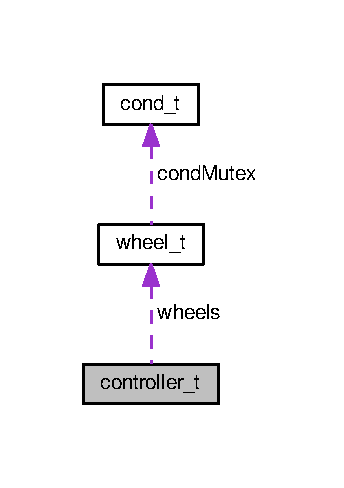
\includegraphics[width=165pt]{structcontroller__t__coll__graph}
\end{center}
\end{figure}
\subsection*{Data Fields}
\begin{DoxyCompactItemize}
\item 
\hyperlink{structwheel__t}{wheel\+\_\+t} \hyperlink{structcontroller__t_a3f7af3fa67cf8e8bfba5ce83ca482139}{wheels} \mbox{[}\hyperlink{struct_threads_8h_ad5e0b1909b281e00eebd4a547a701783}{N\+B\+R\+W\+H\+E\+E\+L\+S}\mbox{]}
\item 
int \hyperlink{structcontroller__t_ab7ad0796d84021de0fd46246b3d5096f}{game\+State}
\item 
int \hyperlink{structcontroller__t_a7fee7b546595edcbee920757b6309386}{win}
\item 
int \hyperlink{structcontroller__t_a3642e8c2aae062cde03de850a554d930}{coins\+Win}
\item 
int \hyperlink{structcontroller__t_ad7b19ae27c8e920ec00b72fb993ebd1e}{coins}
\end{DoxyCompactItemize}


\subsection{Detailed Description}
structure given to the threads, contain all game data 

\subsection{Field Documentation}
\hypertarget{structcontroller__t_ad7b19ae27c8e920ec00b72fb993ebd1e}{\index{controller\+\_\+t@{controller\+\_\+t}!coins@{coins}}
\index{coins@{coins}!controller\+\_\+t@{controller\+\_\+t}}
\subsubsection[{coins}]{\setlength{\rightskip}{0pt plus 5cm}int coins}}\label{structcontroller__t_ad7b19ae27c8e920ec00b72fb993ebd1e}
\hypertarget{structcontroller__t_a3642e8c2aae062cde03de850a554d930}{\index{controller\+\_\+t@{controller\+\_\+t}!coins\+Win@{coins\+Win}}
\index{coins\+Win@{coins\+Win}!controller\+\_\+t@{controller\+\_\+t}}
\subsubsection[{coins\+Win}]{\setlength{\rightskip}{0pt plus 5cm}int coins\+Win}}\label{structcontroller__t_a3642e8c2aae062cde03de850a554d930}
\hypertarget{structcontroller__t_ab7ad0796d84021de0fd46246b3d5096f}{\index{controller\+\_\+t@{controller\+\_\+t}!game\+State@{game\+State}}
\index{game\+State@{game\+State}!controller\+\_\+t@{controller\+\_\+t}}
\subsubsection[{game\+State}]{\setlength{\rightskip}{0pt plus 5cm}int game\+State}}\label{structcontroller__t_ab7ad0796d84021de0fd46246b3d5096f}
\hypertarget{structcontroller__t_a3f7af3fa67cf8e8bfba5ce83ca482139}{\index{controller\+\_\+t@{controller\+\_\+t}!wheels@{wheels}}
\index{wheels@{wheels}!controller\+\_\+t@{controller\+\_\+t}}
\subsubsection[{wheels}]{\setlength{\rightskip}{0pt plus 5cm}{\bf wheel\+\_\+t} wheels\mbox{[}{\bf N\+B\+R\+W\+H\+E\+E\+L\+S}\mbox{]}}}\label{structcontroller__t_a3f7af3fa67cf8e8bfba5ce83ca482139}
\hypertarget{structcontroller__t_a7fee7b546595edcbee920757b6309386}{\index{controller\+\_\+t@{controller\+\_\+t}!win@{win}}
\index{win@{win}!controller\+\_\+t@{controller\+\_\+t}}
\subsubsection[{win}]{\setlength{\rightskip}{0pt plus 5cm}int win}}\label{structcontroller__t_a7fee7b546595edcbee920757b6309386}


The documentation for this struct was generated from the following file\+:\begin{DoxyCompactItemize}
\item 
/home/shinra/\+Clion\+Projects/jackpot/libs/\hyperlink{struct_threads_8h}{struct\+Threads.\+h}\end{DoxyCompactItemize}

\hypertarget{structwheel__t}{\section{wheel\+\_\+t Struct Reference}
\label{structwheel__t}\index{wheel\+\_\+t@{wheel\+\_\+t}}
}


contain \hyperlink{structwheel__t}{wheel\+\_\+t}'s data such as id, current value and time\+Base  




{\ttfamily \#include $<$struct\+Threads.\+h$>$}



Collaboration diagram for wheel\+\_\+t\+:\nopagebreak
\begin{figure}[H]
\begin{center}
\leavevmode
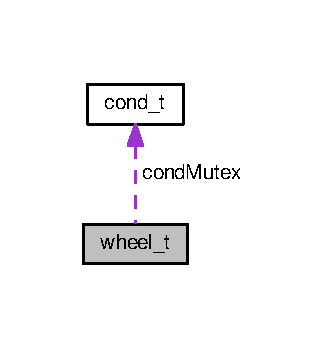
\includegraphics[width=157pt]{structwheel__t__coll__graph}
\end{center}
\end{figure}
\subsection*{Data Fields}
\begin{DoxyCompactItemize}
\item 
int \hyperlink{structwheel__t_a7441ef0865bcb3db9b8064dd7375c1ea}{id}
\item 
int \hyperlink{structwheel__t_ac4f474c82e82cbb89ca7c36dd52be0ed}{value}
\item 
int \hyperlink{structwheel__t_a782adf457267a648e01dbf13d8a16181}{time\+Base}
\item 
\hyperlink{structcond__t}{cond\+\_\+t} $\ast$ \hyperlink{structwheel__t_a24715ed40b477ab5d0426f24cb9e4514}{cond\+Mutex}
\end{DoxyCompactItemize}


\subsection{Detailed Description}
contain \hyperlink{structwheel__t}{wheel\+\_\+t}'s data such as id, current value and time\+Base 

\subsection{Field Documentation}
\hypertarget{structwheel__t_a24715ed40b477ab5d0426f24cb9e4514}{\index{wheel\+\_\+t@{wheel\+\_\+t}!cond\+Mutex@{cond\+Mutex}}
\index{cond\+Mutex@{cond\+Mutex}!wheel\+\_\+t@{wheel\+\_\+t}}
\subsubsection[{cond\+Mutex}]{\setlength{\rightskip}{0pt plus 5cm}{\bf cond\+\_\+t}$\ast$ cond\+Mutex}}\label{structwheel__t_a24715ed40b477ab5d0426f24cb9e4514}
\hypertarget{structwheel__t_a7441ef0865bcb3db9b8064dd7375c1ea}{\index{wheel\+\_\+t@{wheel\+\_\+t}!id@{id}}
\index{id@{id}!wheel\+\_\+t@{wheel\+\_\+t}}
\subsubsection[{id}]{\setlength{\rightskip}{0pt plus 5cm}int id}}\label{structwheel__t_a7441ef0865bcb3db9b8064dd7375c1ea}
\hypertarget{structwheel__t_a782adf457267a648e01dbf13d8a16181}{\index{wheel\+\_\+t@{wheel\+\_\+t}!time\+Base@{time\+Base}}
\index{time\+Base@{time\+Base}!wheel\+\_\+t@{wheel\+\_\+t}}
\subsubsection[{time\+Base}]{\setlength{\rightskip}{0pt plus 5cm}int time\+Base}}\label{structwheel__t_a782adf457267a648e01dbf13d8a16181}
\hypertarget{structwheel__t_ac4f474c82e82cbb89ca7c36dd52be0ed}{\index{wheel\+\_\+t@{wheel\+\_\+t}!value@{value}}
\index{value@{value}!wheel\+\_\+t@{wheel\+\_\+t}}
\subsubsection[{value}]{\setlength{\rightskip}{0pt plus 5cm}int value}}\label{structwheel__t_ac4f474c82e82cbb89ca7c36dd52be0ed}


The documentation for this struct was generated from the following file\+:\begin{DoxyCompactItemize}
\item 
/home/shinra/\+Clion\+Projects/jackpot/libs/\hyperlink{struct_threads_8h}{struct\+Threads.\+h}\end{DoxyCompactItemize}

\chapter{File Documentation}
\hypertarget{display_8c}{\section{/home/shinra/\+Clion\+Projects/jackpot/libs/display.c File Reference}
\label{display_8c}\index{/home/shinra/\+Clion\+Projects/jackpot/libs/display.\+c@{/home/shinra/\+Clion\+Projects/jackpot/libs/display.\+c}}
}


graphic library functions  


{\ttfamily \#include \char`\"{}display.\+h\char`\"{}}\\*
Include dependency graph for display.\+c\+:
\nopagebreak
\begin{figure}[H]
\begin{center}
\leavevmode
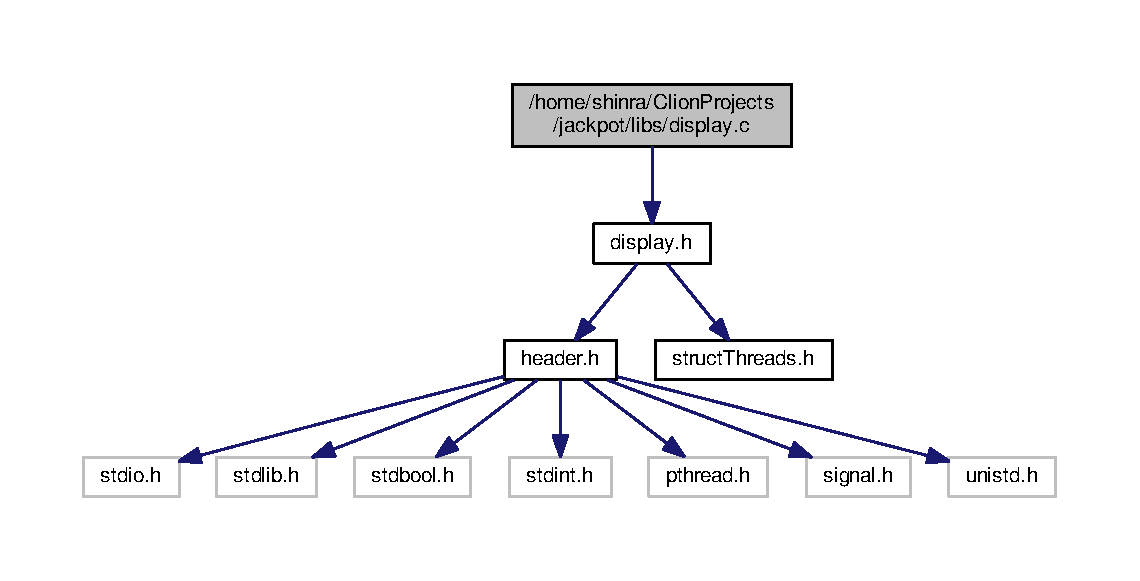
\includegraphics[width=350pt]{display_8c__incl}
\end{center}
\end{figure}
\subsection*{Macros}
\begin{DoxyCompactItemize}
\item 
\#define \hyperlink{display_8c_a5f7e376b50092a15a8a0a831dd9e6d3a}{C\+L\+E\+A\+R\+S\+C\+R\+E\+E\+N}~\char`\"{}\textbackslash{}e\mbox{[}2\+J\char`\"{} /$\ast$$<$! A\+N\+S\+I code to clear the screen $\ast$/
\item 
\#define \hyperlink{display_8c_a45b8baabcef0287684224f3ea7213549}{G\+O\+H\+O\+M\+E}~\char`\"{}\textbackslash{}e\mbox{[}H\char`\"{}  /$\ast$$<$! A\+N\+S\+I code to move the cursor to 0,0 $\ast$/
\end{DoxyCompactItemize}
\subsection*{Functions}
\begin{DoxyCompactItemize}
\item 
void $\ast$ \hyperlink{display_8c_a42cb44b65db3afb21f0e868b54d8b620}{display} (void $\ast$thread\+Data)
\item 
double \hyperlink{display_8c_a3133b3d552d10f6eb3b4178a5531f6f5}{wait\+A\+Frequency} (struct timespec $\ast$start, struct timespec $\ast$\hyperlink{timing_8c_a94ca335b433152f4af4e062084826ae0}{finish}, int frequency)
\end{DoxyCompactItemize}
\subsection*{Variables}
\begin{DoxyCompactItemize}
\item 
const char $\ast$ \hyperlink{display_8c_abc3eab9a64c75eacd405779d3ab6c7c7}{S\+Y\+M\+B\+O\+L\+E\+S} \mbox{[}$\,$\mbox{]} = \{\char`\"{}0\char`\"{},\char`\"{}1\char`\"{},\char`\"{}2\char`\"{},\char`\"{}3\char`\"{},\char`\"{}4\char`\"{},\char`\"{}5\char`\"{},\char`\"{}6\char`\"{},\char`\"{}7\char`\"{},\char`\"{}8\char`\"{},\char`\"{}9\char`\"{}\}
\end{DoxyCompactItemize}


\subsection{Detailed Description}
graphic library functions 

\begin{DoxyAuthor}{Author}
B\+U\+F\+F\+O Pierre, D\+A S\+I\+L\+V\+A Gabriel, M\+E\+H\+M\+E\+D Blazevic 
\end{DoxyAuthor}
\begin{DoxyVersion}{Version}
1.\+0 
\end{DoxyVersion}
\begin{DoxyDate}{Date}
25.\+01.\+2017 
\end{DoxyDate}


\subsection{Macro Definition Documentation}
\hypertarget{display_8c_a5f7e376b50092a15a8a0a831dd9e6d3a}{\index{display.\+c@{display.\+c}!C\+L\+E\+A\+R\+S\+C\+R\+E\+E\+N@{C\+L\+E\+A\+R\+S\+C\+R\+E\+E\+N}}
\index{C\+L\+E\+A\+R\+S\+C\+R\+E\+E\+N@{C\+L\+E\+A\+R\+S\+C\+R\+E\+E\+N}!display.\+c@{display.\+c}}
\subsubsection[{C\+L\+E\+A\+R\+S\+C\+R\+E\+E\+N}]{\setlength{\rightskip}{0pt plus 5cm}\#define C\+L\+E\+A\+R\+S\+C\+R\+E\+E\+N~\char`\"{}\textbackslash{}e\mbox{[}2\+J\char`\"{} /$\ast$$<$! A\+N\+S\+I code to clear the screen $\ast$/}}\label{display_8c_a5f7e376b50092a15a8a0a831dd9e6d3a}
\hypertarget{display_8c_a45b8baabcef0287684224f3ea7213549}{\index{display.\+c@{display.\+c}!G\+O\+H\+O\+M\+E@{G\+O\+H\+O\+M\+E}}
\index{G\+O\+H\+O\+M\+E@{G\+O\+H\+O\+M\+E}!display.\+c@{display.\+c}}
\subsubsection[{G\+O\+H\+O\+M\+E}]{\setlength{\rightskip}{0pt plus 5cm}\#define G\+O\+H\+O\+M\+E~\char`\"{}\textbackslash{}e\mbox{[}H\char`\"{}  /$\ast$$<$! A\+N\+S\+I code to move the cursor to 0,0 $\ast$/}}\label{display_8c_a45b8baabcef0287684224f3ea7213549}


\subsection{Function Documentation}
\hypertarget{display_8c_a42cb44b65db3afb21f0e868b54d8b620}{\index{display.\+c@{display.\+c}!display@{display}}
\index{display@{display}!display.\+c@{display.\+c}}
\subsubsection[{display}]{\setlength{\rightskip}{0pt plus 5cm}void$\ast$ display (
\begin{DoxyParamCaption}
\item[{void $\ast$}]{thread\+Data}
\end{DoxyParamCaption}
)}}\label{display_8c_a42cb44b65db3afb21f0e868b54d8b620}
function given to the display thread 
\begin{DoxyParams}{Parameters}
{\em thread\+Data} & struct containing data to display \\
\hline
\end{DoxyParams}
\begin{DoxyReturn}{Returns}
N\+U\+L\+L 
\end{DoxyReturn}


Here is the call graph for this function\+:\nopagebreak
\begin{figure}[H]
\begin{center}
\leavevmode
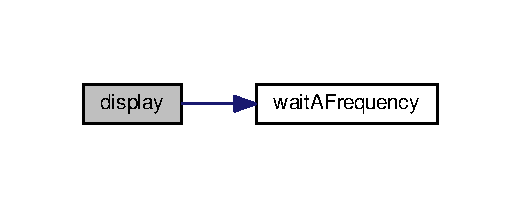
\includegraphics[width=250pt]{display_8c_a42cb44b65db3afb21f0e868b54d8b620_cgraph}
\end{center}
\end{figure}




Here is the caller graph for this function\+:\nopagebreak
\begin{figure}[H]
\begin{center}
\leavevmode
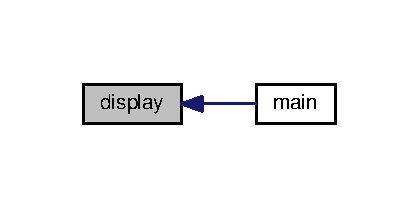
\includegraphics[width=201pt]{display_8c_a42cb44b65db3afb21f0e868b54d8b620_icgraph}
\end{center}
\end{figure}


\hypertarget{display_8c_a3133b3d552d10f6eb3b4178a5531f6f5}{\index{display.\+c@{display.\+c}!wait\+A\+Frequency@{wait\+A\+Frequency}}
\index{wait\+A\+Frequency@{wait\+A\+Frequency}!display.\+c@{display.\+c}}
\subsubsection[{wait\+A\+Frequency}]{\setlength{\rightskip}{0pt plus 5cm}double wait\+A\+Frequency (
\begin{DoxyParamCaption}
\item[{struct timespec $\ast$}]{start, }
\item[{struct timespec $\ast$}]{finish, }
\item[{int}]{frequency}
\end{DoxyParamCaption}
)}}\label{display_8c_a3133b3d552d10f6eb3b4178a5531f6f5}
calculate the time to wait before the next refresh with the time of process 
\begin{DoxyParams}{Parameters}
{\em start} & Start struct with the timer's begin \\
\hline
{\em finish} & Finish struct with the timer's end \\
\hline
{\em frequency} & freq of screen refresh \\
\hline
\end{DoxyParams}
\begin{DoxyReturn}{Returns}
time to wait in nanoseconds or 0 if work process too long 
\end{DoxyReturn}


Here is the caller graph for this function\+:\nopagebreak
\begin{figure}[H]
\begin{center}
\leavevmode
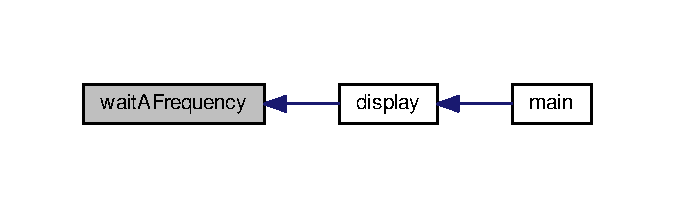
\includegraphics[width=324pt]{display_8c_a3133b3d552d10f6eb3b4178a5531f6f5_icgraph}
\end{center}
\end{figure}




\subsection{Variable Documentation}
\hypertarget{display_8c_abc3eab9a64c75eacd405779d3ab6c7c7}{\index{display.\+c@{display.\+c}!S\+Y\+M\+B\+O\+L\+E\+S@{S\+Y\+M\+B\+O\+L\+E\+S}}
\index{S\+Y\+M\+B\+O\+L\+E\+S@{S\+Y\+M\+B\+O\+L\+E\+S}!display.\+c@{display.\+c}}
\subsubsection[{S\+Y\+M\+B\+O\+L\+E\+S}]{\setlength{\rightskip}{0pt plus 5cm}const char$\ast$ S\+Y\+M\+B\+O\+L\+E\+S\mbox{[}$\,$\mbox{]} = \{\char`\"{}0\char`\"{},\char`\"{}1\char`\"{},\char`\"{}2\char`\"{},\char`\"{}3\char`\"{},\char`\"{}4\char`\"{},\char`\"{}5\char`\"{},\char`\"{}6\char`\"{},\char`\"{}7\char`\"{},\char`\"{}8\char`\"{},\char`\"{}9\char`\"{}\}}}\label{display_8c_abc3eab9a64c75eacd405779d3ab6c7c7}

\hypertarget{display_8h}{\section{/home/shinra/\+Clion\+Projects/jackpot/libs/display.h File Reference}
\label{display_8h}\index{/home/shinra/\+Clion\+Projects/jackpot/libs/display.\+h@{/home/shinra/\+Clion\+Projects/jackpot/libs/display.\+h}}
}


graphic library prototypes  


{\ttfamily \#include \char`\"{}header.\+h\char`\"{}}\\*
{\ttfamily \#include \char`\"{}struct\+Threads.\+h\char`\"{}}\\*
Include dependency graph for display.\+h\+:
\nopagebreak
\begin{figure}[H]
\begin{center}
\leavevmode
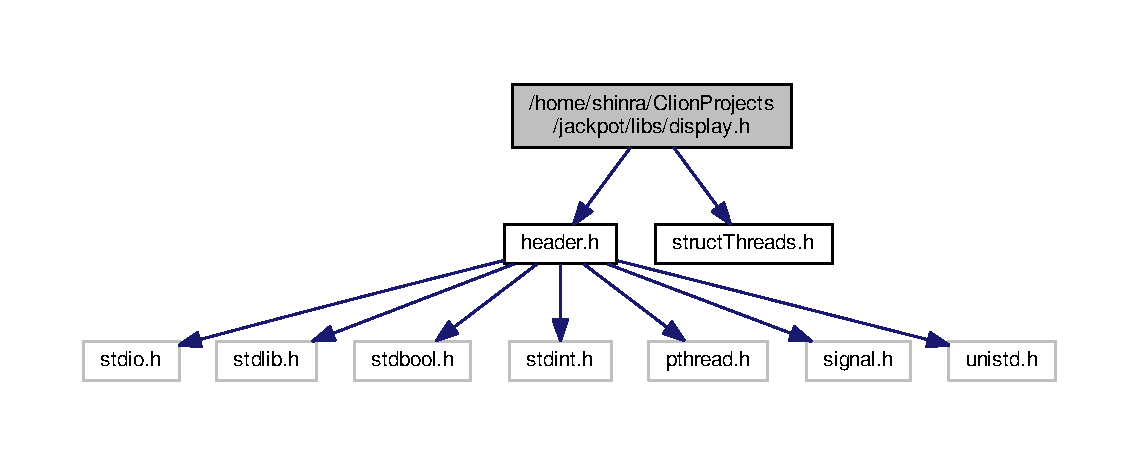
\includegraphics[width=350pt]{display_8h__incl}
\end{center}
\end{figure}
This graph shows which files directly or indirectly include this file\+:\nopagebreak
\begin{figure}[H]
\begin{center}
\leavevmode
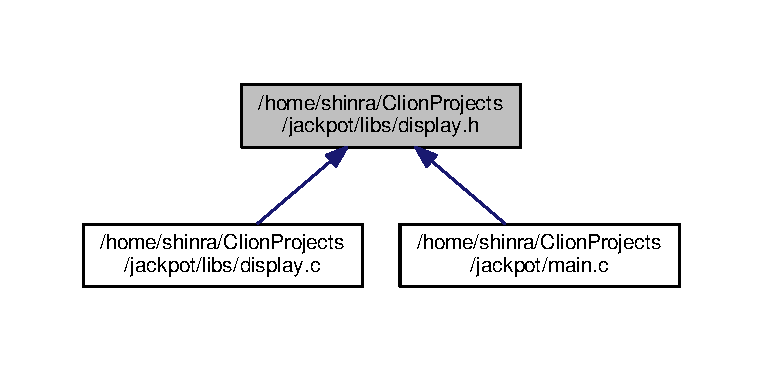
\includegraphics[width=350pt]{display_8h__dep__incl}
\end{center}
\end{figure}
\subsection*{Functions}
\begin{DoxyCompactItemize}
\item 
double \hyperlink{display_8h_a3133b3d552d10f6eb3b4178a5531f6f5}{wait\+A\+Frequency} (struct timespec $\ast$start, struct timespec $\ast$\hyperlink{timing_8c_a94ca335b433152f4af4e062084826ae0}{finish}, int frequency)
\item 
void $\ast$ \hyperlink{display_8h_a42cb44b65db3afb21f0e868b54d8b620}{display} (void $\ast$thread\+Data)
\end{DoxyCompactItemize}


\subsection{Detailed Description}
graphic library prototypes 

\begin{DoxyAuthor}{Author}
B\+U\+F\+F\+O Pierre, D\+A S\+I\+L\+V\+A Gabriel, M\+E\+H\+M\+E\+D Blazevic 
\end{DoxyAuthor}
\begin{DoxyVersion}{Version}
1.\+0 
\end{DoxyVersion}
\begin{DoxyDate}{Date}
25.\+01.\+2017 
\end{DoxyDate}


\subsection{Function Documentation}
\hypertarget{display_8h_a42cb44b65db3afb21f0e868b54d8b620}{\index{display.\+h@{display.\+h}!display@{display}}
\index{display@{display}!display.\+h@{display.\+h}}
\subsubsection[{display}]{\setlength{\rightskip}{0pt plus 5cm}void$\ast$ display (
\begin{DoxyParamCaption}
\item[{void $\ast$}]{thread\+Data}
\end{DoxyParamCaption}
)}}\label{display_8h_a42cb44b65db3afb21f0e868b54d8b620}
function given to the display thread 
\begin{DoxyParams}{Parameters}
{\em thread\+Data} & struct containing data to display \\
\hline
\end{DoxyParams}
\begin{DoxyReturn}{Returns}
N\+U\+L\+L 
\end{DoxyReturn}


Here is the call graph for this function\+:\nopagebreak
\begin{figure}[H]
\begin{center}
\leavevmode
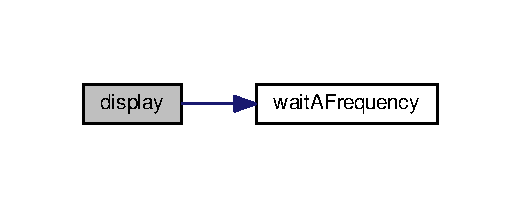
\includegraphics[width=250pt]{display_8h_a42cb44b65db3afb21f0e868b54d8b620_cgraph}
\end{center}
\end{figure}




Here is the caller graph for this function\+:\nopagebreak
\begin{figure}[H]
\begin{center}
\leavevmode
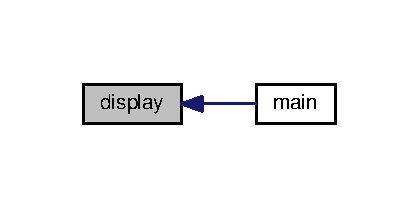
\includegraphics[width=201pt]{display_8h_a42cb44b65db3afb21f0e868b54d8b620_icgraph}
\end{center}
\end{figure}


\hypertarget{display_8h_a3133b3d552d10f6eb3b4178a5531f6f5}{\index{display.\+h@{display.\+h}!wait\+A\+Frequency@{wait\+A\+Frequency}}
\index{wait\+A\+Frequency@{wait\+A\+Frequency}!display.\+h@{display.\+h}}
\subsubsection[{wait\+A\+Frequency}]{\setlength{\rightskip}{0pt plus 5cm}double wait\+A\+Frequency (
\begin{DoxyParamCaption}
\item[{struct timespec $\ast$}]{start, }
\item[{struct timespec $\ast$}]{finish, }
\item[{int}]{frequency}
\end{DoxyParamCaption}
)}}\label{display_8h_a3133b3d552d10f6eb3b4178a5531f6f5}
calculate the time to wait before the next refresh with the time of process 
\begin{DoxyParams}{Parameters}
{\em start} & Start struct with the timer's begin \\
\hline
{\em finish} & Finish struct with the timer's end \\
\hline
{\em frequency} & freq of screen refresh \\
\hline
\end{DoxyParams}
\begin{DoxyReturn}{Returns}
time to wait in nanoseconds or 0 if work process too long 
\end{DoxyReturn}


Here is the caller graph for this function\+:\nopagebreak
\begin{figure}[H]
\begin{center}
\leavevmode
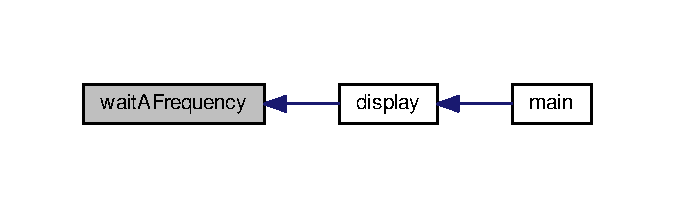
\includegraphics[width=324pt]{display_8h_a3133b3d552d10f6eb3b4178a5531f6f5_icgraph}
\end{center}
\end{figure}



\hypertarget{header_8h}{\section{/home/shinra/\+Clion\+Projects/jackpot/libs/header.h File Reference}
\label{header_8h}\index{/home/shinra/\+Clion\+Projects/jackpot/libs/header.\+h@{/home/shinra/\+Clion\+Projects/jackpot/libs/header.\+h}}
}


files to includes everywhere  


{\ttfamily \#include $<$stdio.\+h$>$}\\*
{\ttfamily \#include $<$stdlib.\+h$>$}\\*
{\ttfamily \#include $<$stdbool.\+h$>$}\\*
{\ttfamily \#include $<$stdint.\+h$>$}\\*
{\ttfamily \#include $<$pthread.\+h$>$}\\*
{\ttfamily \#include $<$signal.\+h$>$}\\*
{\ttfamily \#include $<$unistd.\+h$>$}\\*
Include dependency graph for header.\+h\+:
\nopagebreak
\begin{figure}[H]
\begin{center}
\leavevmode
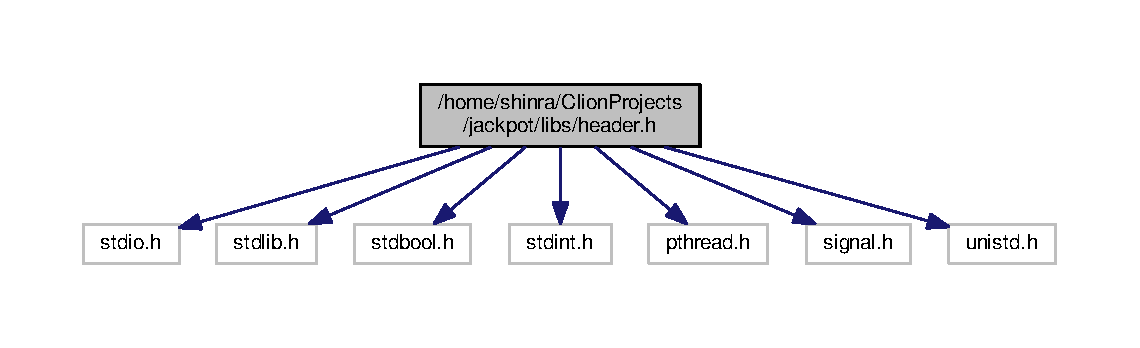
\includegraphics[width=350pt]{header_8h__incl}
\end{center}
\end{figure}
This graph shows which files directly or indirectly include this file\+:\nopagebreak
\begin{figure}[H]
\begin{center}
\leavevmode
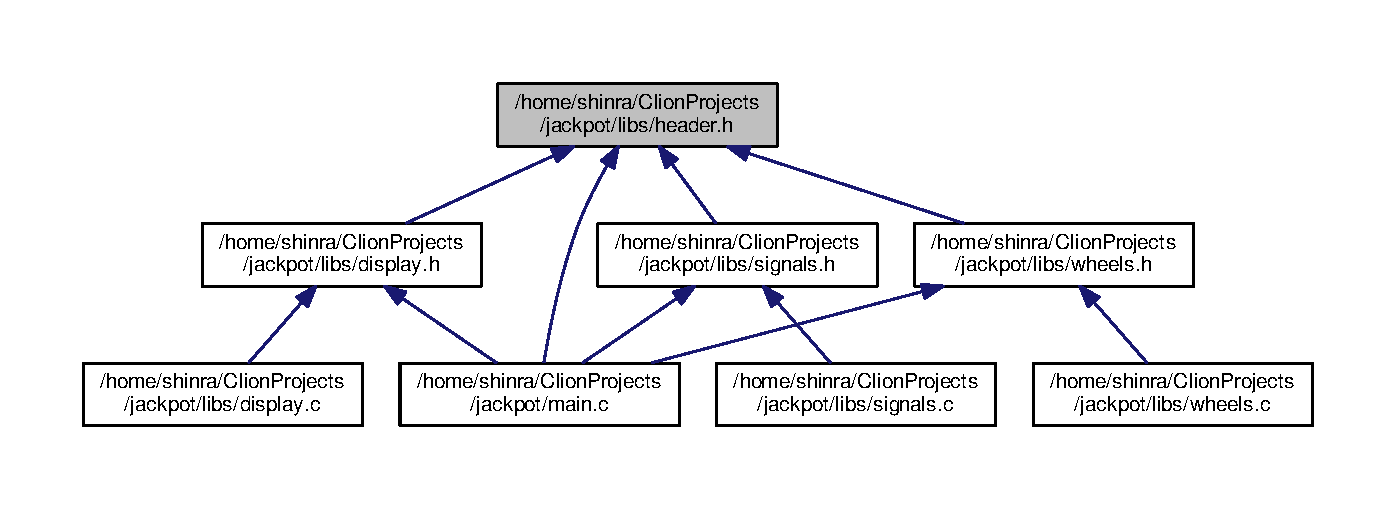
\includegraphics[width=350pt]{header_8h__dep__incl}
\end{center}
\end{figure}
\subsection*{Macros}
\begin{DoxyCompactItemize}
\item 
\#define \hyperlink{header_8h_a369266c24eacffb87046522897a570d5}{\+\_\+\+G\+N\+U\+\_\+\+S\+O\+U\+R\+C\+E}
\end{DoxyCompactItemize}


\subsection{Detailed Description}
files to includes everywhere 

\begin{DoxyAuthor}{Author}
B\+U\+F\+F\+O Pierre, D\+A S\+I\+L\+V\+A Gabriel, M\+E\+H\+M\+E\+D Blazevic 
\end{DoxyAuthor}
\begin{DoxyVersion}{Version}
1.\+0 
\end{DoxyVersion}
\begin{DoxyDate}{Date}
25.\+01.\+2017 
\end{DoxyDate}


\subsection{Macro Definition Documentation}
\hypertarget{header_8h_a369266c24eacffb87046522897a570d5}{\index{header.\+h@{header.\+h}!\+\_\+\+G\+N\+U\+\_\+\+S\+O\+U\+R\+C\+E@{\+\_\+\+G\+N\+U\+\_\+\+S\+O\+U\+R\+C\+E}}
\index{\+\_\+\+G\+N\+U\+\_\+\+S\+O\+U\+R\+C\+E@{\+\_\+\+G\+N\+U\+\_\+\+S\+O\+U\+R\+C\+E}!header.\+h@{header.\+h}}
\subsubsection[{\+\_\+\+G\+N\+U\+\_\+\+S\+O\+U\+R\+C\+E}]{\setlength{\rightskip}{0pt plus 5cm}\#define \+\_\+\+G\+N\+U\+\_\+\+S\+O\+U\+R\+C\+E}}\label{header_8h_a369266c24eacffb87046522897a570d5}

\hypertarget{signals_8c}{\section{/home/shinra/\+Clion\+Projects/jackpot/libs/signals.c File Reference}
\label{signals_8c}\index{/home/shinra/\+Clion\+Projects/jackpot/libs/signals.\+c@{/home/shinra/\+Clion\+Projects/jackpot/libs/signals.\+c}}
}


signals library  


{\ttfamily \#include \char`\"{}signals.\+h\char`\"{}}\\*
Include dependency graph for signals.\+c\+:
\nopagebreak
\begin{figure}[H]
\begin{center}
\leavevmode
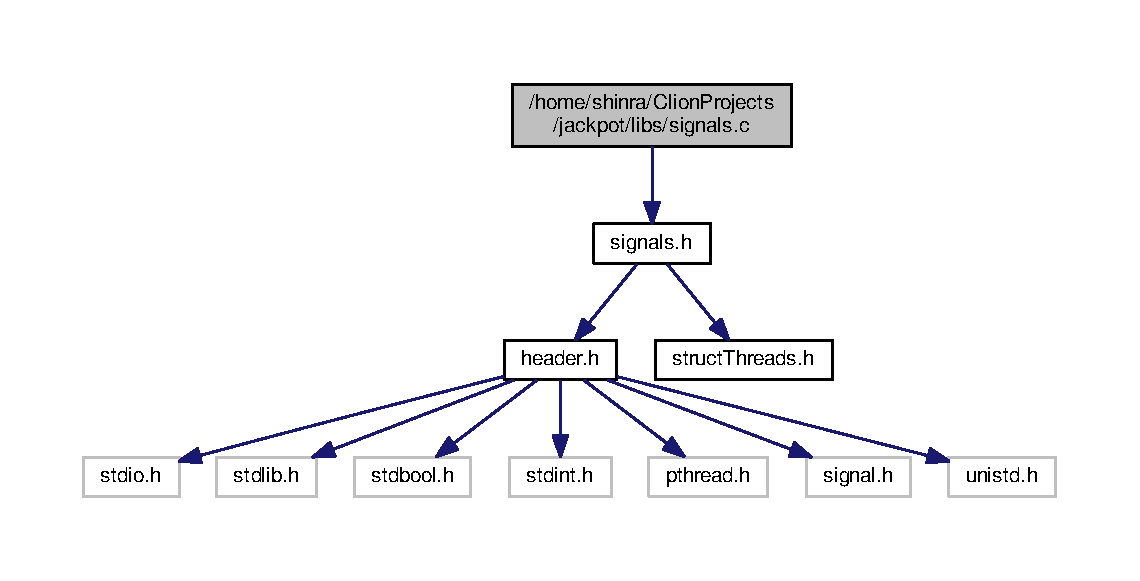
\includegraphics[width=350pt]{signals_8c__incl}
\end{center}
\end{figure}
\subsection*{Functions}
\begin{DoxyCompactItemize}
\item 
void $\ast$ \hyperlink{signals_8c_a6e85cf2c8ee979e0310b5912ec10307b}{signal\+Receiver} (void $\ast$thread\+Data)
\end{DoxyCompactItemize}


\subsection{Detailed Description}
signals library 

\begin{DoxyAuthor}{Author}
B\+U\+F\+F\+O Pierre, D\+A S\+I\+L\+V\+A Gabriel, M\+E\+H\+M\+E\+D Blazevic 
\end{DoxyAuthor}
\begin{DoxyVersion}{Version}
1.\+0 
\end{DoxyVersion}
\begin{DoxyDate}{Date}
25.\+01.\+2017 
\end{DoxyDate}


\subsection{Function Documentation}
\hypertarget{signals_8c_a6e85cf2c8ee979e0310b5912ec10307b}{\index{signals.\+c@{signals.\+c}!signal\+Receiver@{signal\+Receiver}}
\index{signal\+Receiver@{signal\+Receiver}!signals.\+c@{signals.\+c}}
\subsubsection[{signal\+Receiver}]{\setlength{\rightskip}{0pt plus 5cm}void$\ast$ signal\+Receiver (
\begin{DoxyParamCaption}
\item[{void $\ast$}]{thread\+Data}
\end{DoxyParamCaption}
)}}\label{signals_8c_a6e85cf2c8ee979e0310b5912ec10307b}
thread which control the signals received, here we use 4 signals\+: S\+I\+G\+I\+N\+T,S\+I\+G\+T\+S\+T\+P, S\+I\+G\+Q\+U\+I\+T and S\+I\+G\+A\+L\+R\+M 
\begin{DoxyParams}{Parameters}
{\em thread\+Data} & -\/ struct containing the datas \\
\hline
\end{DoxyParams}
\begin{DoxyReturn}{Returns}
N\+U\+L\+L 
\end{DoxyReturn}


Here is the caller graph for this function\+:\nopagebreak
\begin{figure}[H]
\begin{center}
\leavevmode
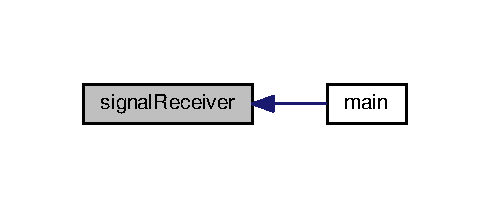
\includegraphics[width=235pt]{signals_8c_a6e85cf2c8ee979e0310b5912ec10307b_icgraph}
\end{center}
\end{figure}



\hypertarget{signals_8h}{\section{/home/shinra/\+Clion\+Projects/jackpot/libs/signals.h File Reference}
\label{signals_8h}\index{/home/shinra/\+Clion\+Projects/jackpot/libs/signals.\+h@{/home/shinra/\+Clion\+Projects/jackpot/libs/signals.\+h}}
}


signals library  


{\ttfamily \#include \char`\"{}header.\+h\char`\"{}}\\*
{\ttfamily \#include \char`\"{}struct\+Threads.\+h\char`\"{}}\\*
Include dependency graph for signals.\+h\+:
\nopagebreak
\begin{figure}[H]
\begin{center}
\leavevmode
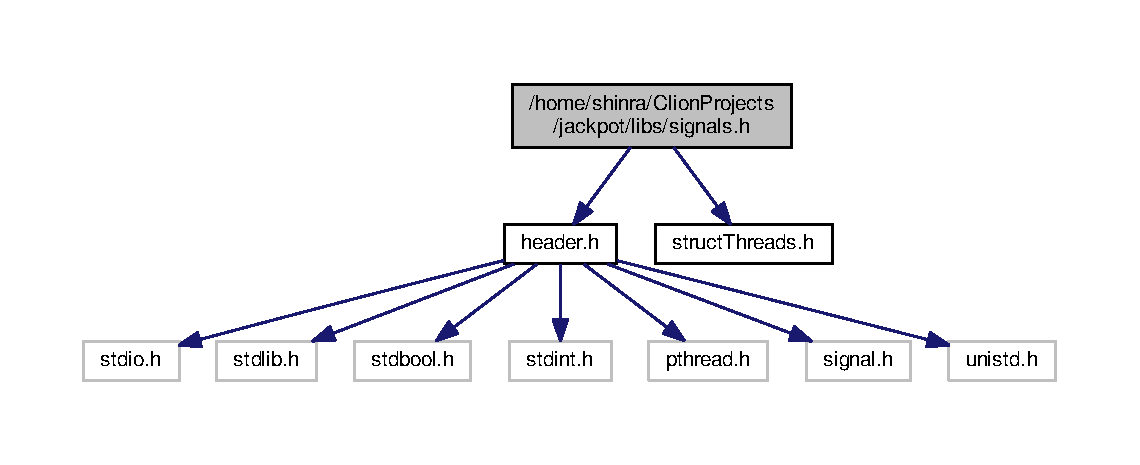
\includegraphics[width=350pt]{signals_8h__incl}
\end{center}
\end{figure}
This graph shows which files directly or indirectly include this file\+:\nopagebreak
\begin{figure}[H]
\begin{center}
\leavevmode
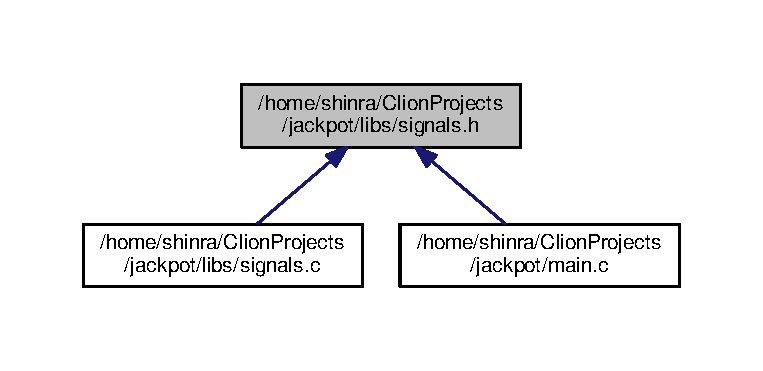
\includegraphics[width=350pt]{signals_8h__dep__incl}
\end{center}
\end{figure}
\subsection*{Functions}
\begin{DoxyCompactItemize}
\item 
void $\ast$ \hyperlink{signals_8h_a6e85cf2c8ee979e0310b5912ec10307b}{signal\+Receiver} (void $\ast$thread\+Data)
\item 
void $\ast$ \hyperlink{signals_8h_a29545553789ce46345079f62ed936ad0}{timer} (void $\ast$thread\+Data)
\end{DoxyCompactItemize}


\subsection{Detailed Description}
signals library 

\begin{DoxyAuthor}{Author}
B\+U\+F\+F\+O Pierre, D\+A S\+I\+L\+V\+A Gabriel, M\+E\+H\+M\+E\+D Blazevic 
\end{DoxyAuthor}
\begin{DoxyVersion}{Version}
1.\+0 
\end{DoxyVersion}
\begin{DoxyDate}{Date}
25.\+01.\+2017 
\end{DoxyDate}


\subsection{Function Documentation}
\hypertarget{signals_8h_a6e85cf2c8ee979e0310b5912ec10307b}{\index{signals.\+h@{signals.\+h}!signal\+Receiver@{signal\+Receiver}}
\index{signal\+Receiver@{signal\+Receiver}!signals.\+h@{signals.\+h}}
\subsubsection[{signal\+Receiver}]{\setlength{\rightskip}{0pt plus 5cm}void$\ast$ signal\+Receiver (
\begin{DoxyParamCaption}
\item[{void $\ast$}]{thread\+Data}
\end{DoxyParamCaption}
)}}\label{signals_8h_a6e85cf2c8ee979e0310b5912ec10307b}
thread which control the signals received, here we use 4 signals\+: S\+I\+G\+I\+N\+T,S\+I\+G\+T\+S\+T\+P, S\+I\+G\+Q\+U\+I\+T and S\+I\+G\+A\+L\+R\+M 
\begin{DoxyParams}{Parameters}
{\em thread\+Data} & -\/ struct containing the datas \\
\hline
\end{DoxyParams}
\begin{DoxyReturn}{Returns}
N\+U\+L\+L 
\end{DoxyReturn}


Here is the caller graph for this function\+:
\nopagebreak
\begin{figure}[H]
\begin{center}
\leavevmode
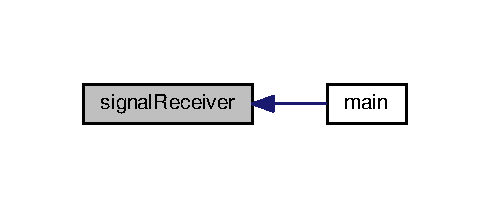
\includegraphics[width=235pt]{signals_8h_a6e85cf2c8ee979e0310b5912ec10307b_icgraph}
\end{center}
\end{figure}


\hypertarget{signals_8h_a29545553789ce46345079f62ed936ad0}{\index{signals.\+h@{signals.\+h}!timer@{timer}}
\index{timer@{timer}!signals.\+h@{signals.\+h}}
\subsubsection[{timer}]{\setlength{\rightskip}{0pt plus 5cm}void$\ast$ timer (
\begin{DoxyParamCaption}
\item[{void $\ast$}]{thread\+Data}
\end{DoxyParamCaption}
)}}\label{signals_8h_a29545553789ce46345079f62ed936ad0}

\hypertarget{struct_threads_8h}{\section{/home/shinra/\+Clion\+Projects/jackpot/libs/struct\+Threads.h File Reference}
\label{struct_threads_8h}\index{/home/shinra/\+Clion\+Projects/jackpot/libs/struct\+Threads.\+h@{/home/shinra/\+Clion\+Projects/jackpot/libs/struct\+Threads.\+h}}
}


threads struct and constants  


This graph shows which files directly or indirectly include this file\+:\nopagebreak
\begin{figure}[H]
\begin{center}
\leavevmode
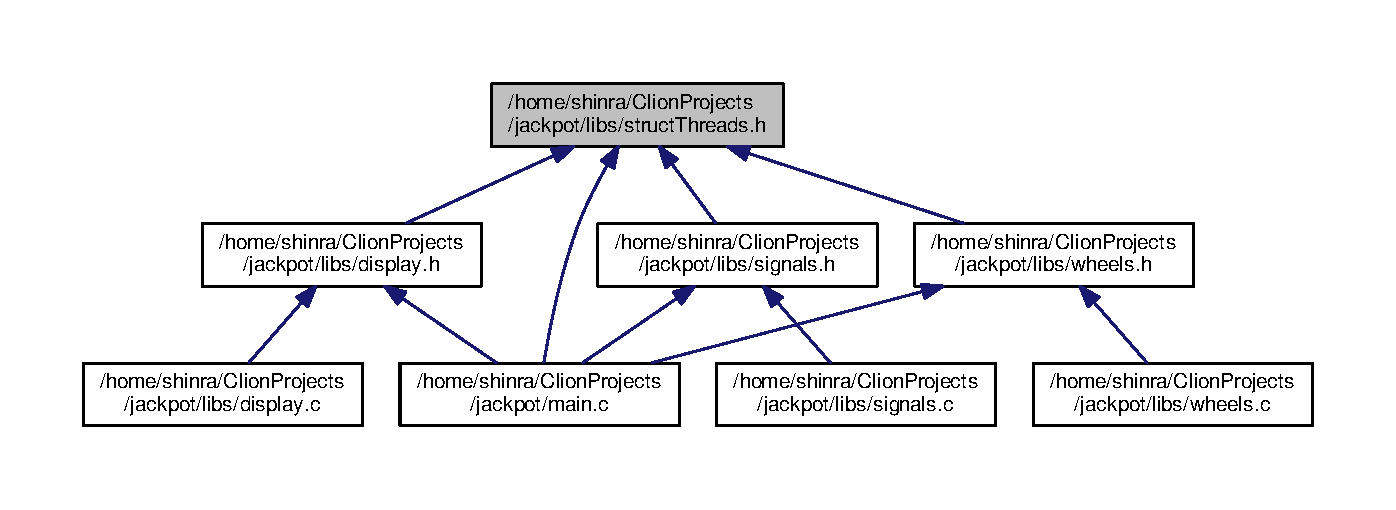
\includegraphics[width=350pt]{struct_threads_8h__dep__incl}
\end{center}
\end{figure}
\subsection*{Data Structures}
\begin{DoxyCompactItemize}
\item 
struct \hyperlink{structcond__t}{cond\+\_\+t}
\item 
struct \hyperlink{structwheel__t}{wheel\+\_\+t}
\begin{DoxyCompactList}\small\item\em contain \hyperlink{structwheel__t}{wheel\+\_\+t}'s data such as id, current value and time\+Base \end{DoxyCompactList}\item 
struct \hyperlink{structcontroller__t}{controller\+\_\+t}
\begin{DoxyCompactList}\small\item\em structure given to the threads, contain all game data \end{DoxyCompactList}\end{DoxyCompactItemize}
\subsection*{Macros}
\begin{DoxyCompactItemize}
\item 
\#define \hyperlink{struct_threads_8h_ad5e0b1909b281e00eebd4a547a701783}{N\+B\+R\+W\+H\+E\+E\+L\+S}~3
\item 
\#define \hyperlink{struct_threads_8h_a3007a56adab27c692a4248ebe74ed57a}{N\+R\+B\+S\+Y\+M\+B\+O\+L\+S}~10
\item 
\#define \hyperlink{struct_threads_8h_acbb179521c70d42fff68a9c6305c7450}{B\+A\+S\+E\+T\+I\+M\+E}~12000
\item 
\#define \hyperlink{struct_threads_8h_a84142cd3e3bf14c4ecd4b6707a808c39}{F\+R\+E\+Q\+U\+E\+N\+C\+Y}~30
\item 
\#define \hyperlink{struct_threads_8h_afa02536da133d78c6e2c6703ae4c4805}{I\+N\+I\+T\+I\+A\+L\+A\+N\+T\+E}~1
\item 
\#define \hyperlink{struct_threads_8h_adb0f9c21a49628a9f5d03175ead4d05e}{I\+N\+I\+T\+I\+A\+L\+C\+O\+I\+N\+S}~10
\item 
\#define \hyperlink{struct_threads_8h_a13ee57d95da6b6509d43bb1b3f67bb02}{W\+A\+I\+T\+I\+N\+G}~0
\item 
\#define \hyperlink{struct_threads_8h_aa1eb38e9057fad2d3d88a7e4cdc52edd}{R\+O\+L\+L\+I\+N\+G}~1
\item 
\#define \hyperlink{struct_threads_8h_a6a1e3fd193b6dd39939b3c436d1014ce}{F\+I\+N\+I\+S\+H\+E\+D}~2
\item 
\#define \hyperlink{struct_threads_8h_ae8d47456e9bc5e294fa07798c66c2070}{E\+N\+D\+M\+S\+G}~3
\item 
\#define \hyperlink{struct_threads_8h_a0d781d111f2907153eb8fd334b4495eb}{L\+O\+S\+T}~0
\item 
\#define \hyperlink{struct_threads_8h_aa95a923bab80ed6e3577cab94d2e2ed2}{D\+O\+U\+B\+L\+E\+W\+I\+N}~1
\item 
\#define \hyperlink{struct_threads_8h_a991c4bb0231e5d368ef05cae01bf5b70}{F\+U\+L\+L\+W\+I\+N}~2
\item 
\#define \hyperlink{struct_threads_8h_a4e60d0e15b9cdf0401619dc23829de69}{F\+I\+N\+I\+S\+H\+E\+D\+P\+R\+O\+G\+R\+A\+M}~-\/1
\item 
\#define \hyperlink{struct_threads_8h_a797c6452bfab76ee0986efc721ae01b4}{T\+I\+M\+E\+B\+E\+F\+O\+R\+E\+W\+H\+E\+E\+L\+T\+I\+M\+O\+U\+T}~3
\end{DoxyCompactItemize}
\subsection*{Typedefs}
\begin{DoxyCompactItemize}
\item 
typedef struct \hyperlink{structcond__t}{cond\+\_\+t} \hyperlink{struct_threads_8h_a1c22c315a1fc72a4dbccb916f3c1e4aa}{cond\+\_\+t}
\item 
typedef struct \hyperlink{structwheel__t}{wheel\+\_\+t} \hyperlink{struct_threads_8h_ac5b6533c9edcdcd6d280a1df804ed025}{wheel\+\_\+t}
\item 
typedef struct \hyperlink{structcontroller__t}{controller\+\_\+t} \hyperlink{struct_threads_8h_ac13ee0500b8913123a6a97b586c5a53c}{controller\+\_\+t}
\end{DoxyCompactItemize}


\subsection{Detailed Description}
threads struct and constants 

\begin{DoxyAuthor}{Author}
B\+U\+F\+F\+O Pierre, D\+A S\+I\+L\+V\+A Gabriel, M\+E\+H\+M\+E\+D Blazevic 
\end{DoxyAuthor}
\begin{DoxyVersion}{Version}
1.\+0 
\end{DoxyVersion}
\begin{DoxyDate}{Date}
25.\+01.\+2017 
\end{DoxyDate}


\subsection{Macro Definition Documentation}
\hypertarget{struct_threads_8h_acbb179521c70d42fff68a9c6305c7450}{\index{struct\+Threads.\+h@{struct\+Threads.\+h}!B\+A\+S\+E\+T\+I\+M\+E@{B\+A\+S\+E\+T\+I\+M\+E}}
\index{B\+A\+S\+E\+T\+I\+M\+E@{B\+A\+S\+E\+T\+I\+M\+E}!struct\+Threads.\+h@{struct\+Threads.\+h}}
\subsubsection[{B\+A\+S\+E\+T\+I\+M\+E}]{\setlength{\rightskip}{0pt plus 5cm}\#define B\+A\+S\+E\+T\+I\+M\+E~12000}}\label{struct_threads_8h_acbb179521c70d42fff68a9c6305c7450}
\hypertarget{struct_threads_8h_aa95a923bab80ed6e3577cab94d2e2ed2}{\index{struct\+Threads.\+h@{struct\+Threads.\+h}!D\+O\+U\+B\+L\+E\+W\+I\+N@{D\+O\+U\+B\+L\+E\+W\+I\+N}}
\index{D\+O\+U\+B\+L\+E\+W\+I\+N@{D\+O\+U\+B\+L\+E\+W\+I\+N}!struct\+Threads.\+h@{struct\+Threads.\+h}}
\subsubsection[{D\+O\+U\+B\+L\+E\+W\+I\+N}]{\setlength{\rightskip}{0pt plus 5cm}\#define D\+O\+U\+B\+L\+E\+W\+I\+N~1}}\label{struct_threads_8h_aa95a923bab80ed6e3577cab94d2e2ed2}
\hypertarget{struct_threads_8h_ae8d47456e9bc5e294fa07798c66c2070}{\index{struct\+Threads.\+h@{struct\+Threads.\+h}!E\+N\+D\+M\+S\+G@{E\+N\+D\+M\+S\+G}}
\index{E\+N\+D\+M\+S\+G@{E\+N\+D\+M\+S\+G}!struct\+Threads.\+h@{struct\+Threads.\+h}}
\subsubsection[{E\+N\+D\+M\+S\+G}]{\setlength{\rightskip}{0pt plus 5cm}\#define E\+N\+D\+M\+S\+G~3}}\label{struct_threads_8h_ae8d47456e9bc5e294fa07798c66c2070}
\hypertarget{struct_threads_8h_a6a1e3fd193b6dd39939b3c436d1014ce}{\index{struct\+Threads.\+h@{struct\+Threads.\+h}!F\+I\+N\+I\+S\+H\+E\+D@{F\+I\+N\+I\+S\+H\+E\+D}}
\index{F\+I\+N\+I\+S\+H\+E\+D@{F\+I\+N\+I\+S\+H\+E\+D}!struct\+Threads.\+h@{struct\+Threads.\+h}}
\subsubsection[{F\+I\+N\+I\+S\+H\+E\+D}]{\setlength{\rightskip}{0pt plus 5cm}\#define F\+I\+N\+I\+S\+H\+E\+D~2}}\label{struct_threads_8h_a6a1e3fd193b6dd39939b3c436d1014ce}
\hypertarget{struct_threads_8h_a4e60d0e15b9cdf0401619dc23829de69}{\index{struct\+Threads.\+h@{struct\+Threads.\+h}!F\+I\+N\+I\+S\+H\+E\+D\+P\+R\+O\+G\+R\+A\+M@{F\+I\+N\+I\+S\+H\+E\+D\+P\+R\+O\+G\+R\+A\+M}}
\index{F\+I\+N\+I\+S\+H\+E\+D\+P\+R\+O\+G\+R\+A\+M@{F\+I\+N\+I\+S\+H\+E\+D\+P\+R\+O\+G\+R\+A\+M}!struct\+Threads.\+h@{struct\+Threads.\+h}}
\subsubsection[{F\+I\+N\+I\+S\+H\+E\+D\+P\+R\+O\+G\+R\+A\+M}]{\setlength{\rightskip}{0pt plus 5cm}\#define F\+I\+N\+I\+S\+H\+E\+D\+P\+R\+O\+G\+R\+A\+M~-\/1}}\label{struct_threads_8h_a4e60d0e15b9cdf0401619dc23829de69}
\hypertarget{struct_threads_8h_a84142cd3e3bf14c4ecd4b6707a808c39}{\index{struct\+Threads.\+h@{struct\+Threads.\+h}!F\+R\+E\+Q\+U\+E\+N\+C\+Y@{F\+R\+E\+Q\+U\+E\+N\+C\+Y}}
\index{F\+R\+E\+Q\+U\+E\+N\+C\+Y@{F\+R\+E\+Q\+U\+E\+N\+C\+Y}!struct\+Threads.\+h@{struct\+Threads.\+h}}
\subsubsection[{F\+R\+E\+Q\+U\+E\+N\+C\+Y}]{\setlength{\rightskip}{0pt plus 5cm}\#define F\+R\+E\+Q\+U\+E\+N\+C\+Y~30}}\label{struct_threads_8h_a84142cd3e3bf14c4ecd4b6707a808c39}
\hypertarget{struct_threads_8h_a991c4bb0231e5d368ef05cae01bf5b70}{\index{struct\+Threads.\+h@{struct\+Threads.\+h}!F\+U\+L\+L\+W\+I\+N@{F\+U\+L\+L\+W\+I\+N}}
\index{F\+U\+L\+L\+W\+I\+N@{F\+U\+L\+L\+W\+I\+N}!struct\+Threads.\+h@{struct\+Threads.\+h}}
\subsubsection[{F\+U\+L\+L\+W\+I\+N}]{\setlength{\rightskip}{0pt plus 5cm}\#define F\+U\+L\+L\+W\+I\+N~2}}\label{struct_threads_8h_a991c4bb0231e5d368ef05cae01bf5b70}
\hypertarget{struct_threads_8h_afa02536da133d78c6e2c6703ae4c4805}{\index{struct\+Threads.\+h@{struct\+Threads.\+h}!I\+N\+I\+T\+I\+A\+L\+A\+N\+T\+E@{I\+N\+I\+T\+I\+A\+L\+A\+N\+T\+E}}
\index{I\+N\+I\+T\+I\+A\+L\+A\+N\+T\+E@{I\+N\+I\+T\+I\+A\+L\+A\+N\+T\+E}!struct\+Threads.\+h@{struct\+Threads.\+h}}
\subsubsection[{I\+N\+I\+T\+I\+A\+L\+A\+N\+T\+E}]{\setlength{\rightskip}{0pt plus 5cm}\#define I\+N\+I\+T\+I\+A\+L\+A\+N\+T\+E~1}}\label{struct_threads_8h_afa02536da133d78c6e2c6703ae4c4805}
\hypertarget{struct_threads_8h_adb0f9c21a49628a9f5d03175ead4d05e}{\index{struct\+Threads.\+h@{struct\+Threads.\+h}!I\+N\+I\+T\+I\+A\+L\+C\+O\+I\+N\+S@{I\+N\+I\+T\+I\+A\+L\+C\+O\+I\+N\+S}}
\index{I\+N\+I\+T\+I\+A\+L\+C\+O\+I\+N\+S@{I\+N\+I\+T\+I\+A\+L\+C\+O\+I\+N\+S}!struct\+Threads.\+h@{struct\+Threads.\+h}}
\subsubsection[{I\+N\+I\+T\+I\+A\+L\+C\+O\+I\+N\+S}]{\setlength{\rightskip}{0pt plus 5cm}\#define I\+N\+I\+T\+I\+A\+L\+C\+O\+I\+N\+S~10}}\label{struct_threads_8h_adb0f9c21a49628a9f5d03175ead4d05e}
\hypertarget{struct_threads_8h_a0d781d111f2907153eb8fd334b4495eb}{\index{struct\+Threads.\+h@{struct\+Threads.\+h}!L\+O\+S\+T@{L\+O\+S\+T}}
\index{L\+O\+S\+T@{L\+O\+S\+T}!struct\+Threads.\+h@{struct\+Threads.\+h}}
\subsubsection[{L\+O\+S\+T}]{\setlength{\rightskip}{0pt plus 5cm}\#define L\+O\+S\+T~0}}\label{struct_threads_8h_a0d781d111f2907153eb8fd334b4495eb}
\hypertarget{struct_threads_8h_ad5e0b1909b281e00eebd4a547a701783}{\index{struct\+Threads.\+h@{struct\+Threads.\+h}!N\+B\+R\+W\+H\+E\+E\+L\+S@{N\+B\+R\+W\+H\+E\+E\+L\+S}}
\index{N\+B\+R\+W\+H\+E\+E\+L\+S@{N\+B\+R\+W\+H\+E\+E\+L\+S}!struct\+Threads.\+h@{struct\+Threads.\+h}}
\subsubsection[{N\+B\+R\+W\+H\+E\+E\+L\+S}]{\setlength{\rightskip}{0pt plus 5cm}\#define N\+B\+R\+W\+H\+E\+E\+L\+S~3}}\label{struct_threads_8h_ad5e0b1909b281e00eebd4a547a701783}
\hypertarget{struct_threads_8h_a3007a56adab27c692a4248ebe74ed57a}{\index{struct\+Threads.\+h@{struct\+Threads.\+h}!N\+R\+B\+S\+Y\+M\+B\+O\+L\+S@{N\+R\+B\+S\+Y\+M\+B\+O\+L\+S}}
\index{N\+R\+B\+S\+Y\+M\+B\+O\+L\+S@{N\+R\+B\+S\+Y\+M\+B\+O\+L\+S}!struct\+Threads.\+h@{struct\+Threads.\+h}}
\subsubsection[{N\+R\+B\+S\+Y\+M\+B\+O\+L\+S}]{\setlength{\rightskip}{0pt plus 5cm}\#define N\+R\+B\+S\+Y\+M\+B\+O\+L\+S~10}}\label{struct_threads_8h_a3007a56adab27c692a4248ebe74ed57a}
\hypertarget{struct_threads_8h_aa1eb38e9057fad2d3d88a7e4cdc52edd}{\index{struct\+Threads.\+h@{struct\+Threads.\+h}!R\+O\+L\+L\+I\+N\+G@{R\+O\+L\+L\+I\+N\+G}}
\index{R\+O\+L\+L\+I\+N\+G@{R\+O\+L\+L\+I\+N\+G}!struct\+Threads.\+h@{struct\+Threads.\+h}}
\subsubsection[{R\+O\+L\+L\+I\+N\+G}]{\setlength{\rightskip}{0pt plus 5cm}\#define R\+O\+L\+L\+I\+N\+G~1}}\label{struct_threads_8h_aa1eb38e9057fad2d3d88a7e4cdc52edd}
\hypertarget{struct_threads_8h_a797c6452bfab76ee0986efc721ae01b4}{\index{struct\+Threads.\+h@{struct\+Threads.\+h}!T\+I\+M\+E\+B\+E\+F\+O\+R\+E\+W\+H\+E\+E\+L\+T\+I\+M\+O\+U\+T@{T\+I\+M\+E\+B\+E\+F\+O\+R\+E\+W\+H\+E\+E\+L\+T\+I\+M\+O\+U\+T}}
\index{T\+I\+M\+E\+B\+E\+F\+O\+R\+E\+W\+H\+E\+E\+L\+T\+I\+M\+O\+U\+T@{T\+I\+M\+E\+B\+E\+F\+O\+R\+E\+W\+H\+E\+E\+L\+T\+I\+M\+O\+U\+T}!struct\+Threads.\+h@{struct\+Threads.\+h}}
\subsubsection[{T\+I\+M\+E\+B\+E\+F\+O\+R\+E\+W\+H\+E\+E\+L\+T\+I\+M\+O\+U\+T}]{\setlength{\rightskip}{0pt plus 5cm}\#define T\+I\+M\+E\+B\+E\+F\+O\+R\+E\+W\+H\+E\+E\+L\+T\+I\+M\+O\+U\+T~3}}\label{struct_threads_8h_a797c6452bfab76ee0986efc721ae01b4}
\hypertarget{struct_threads_8h_a13ee57d95da6b6509d43bb1b3f67bb02}{\index{struct\+Threads.\+h@{struct\+Threads.\+h}!W\+A\+I\+T\+I\+N\+G@{W\+A\+I\+T\+I\+N\+G}}
\index{W\+A\+I\+T\+I\+N\+G@{W\+A\+I\+T\+I\+N\+G}!struct\+Threads.\+h@{struct\+Threads.\+h}}
\subsubsection[{W\+A\+I\+T\+I\+N\+G}]{\setlength{\rightskip}{0pt plus 5cm}\#define W\+A\+I\+T\+I\+N\+G~0}}\label{struct_threads_8h_a13ee57d95da6b6509d43bb1b3f67bb02}


\subsection{Typedef Documentation}
\hypertarget{struct_threads_8h_a1c22c315a1fc72a4dbccb916f3c1e4aa}{\index{struct\+Threads.\+h@{struct\+Threads.\+h}!cond\+\_\+t@{cond\+\_\+t}}
\index{cond\+\_\+t@{cond\+\_\+t}!struct\+Threads.\+h@{struct\+Threads.\+h}}
\subsubsection[{cond\+\_\+t}]{\setlength{\rightskip}{0pt plus 5cm}typedef struct {\bf cond\+\_\+t} {\bf cond\+\_\+t}}}\label{struct_threads_8h_a1c22c315a1fc72a4dbccb916f3c1e4aa}
\hypertarget{struct_threads_8h_ac13ee0500b8913123a6a97b586c5a53c}{\index{struct\+Threads.\+h@{struct\+Threads.\+h}!controller\+\_\+t@{controller\+\_\+t}}
\index{controller\+\_\+t@{controller\+\_\+t}!struct\+Threads.\+h@{struct\+Threads.\+h}}
\subsubsection[{controller\+\_\+t}]{\setlength{\rightskip}{0pt plus 5cm}typedef struct {\bf controller\+\_\+t}  {\bf controller\+\_\+t}}}\label{struct_threads_8h_ac13ee0500b8913123a6a97b586c5a53c}
\hypertarget{struct_threads_8h_ac5b6533c9edcdcd6d280a1df804ed025}{\index{struct\+Threads.\+h@{struct\+Threads.\+h}!wheel\+\_\+t@{wheel\+\_\+t}}
\index{wheel\+\_\+t@{wheel\+\_\+t}!struct\+Threads.\+h@{struct\+Threads.\+h}}
\subsubsection[{wheel\+\_\+t}]{\setlength{\rightskip}{0pt plus 5cm}typedef struct {\bf wheel\+\_\+t}  {\bf wheel\+\_\+t}}}\label{struct_threads_8h_ac5b6533c9edcdcd6d280a1df804ed025}

\hypertarget{timing_8c}{\section{/home/shinra/\+Clion\+Projects/jackpot/libs/timing.c File Reference}
\label{timing_8c}\index{/home/shinra/\+Clion\+Projects/jackpot/libs/timing.\+c@{/home/shinra/\+Clion\+Projects/jackpot/libs/timing.\+c}}
}


timing's functions, allows the user to count the time in secondes, between a start and a stop call.  


{\ttfamily \#include \char`\"{}timing.\+h\char`\"{}}\\*
Include dependency graph for timing.\+c\+:\nopagebreak
\begin{figure}[H]
\begin{center}
\leavevmode
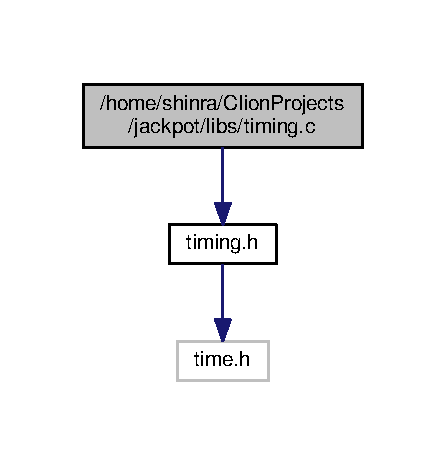
\includegraphics[width=214pt]{timing_8c__incl}
\end{center}
\end{figure}
\subsection*{Functions}
\begin{DoxyCompactItemize}
\item 
void \hyperlink{timing_8c_a606c0b10d8a2b94f79b1d273d2532db0}{start\+Time} ()
\item 
void \hyperlink{timing_8c_af5f394416f4d08f504e88587f60cc489}{stop\+Time} ()
\item 
double \hyperlink{timing_8c_ac56c08903fe71f3197168456aef26524}{get\+Cnt\+Time} ()
\end{DoxyCompactItemize}
\subsection*{Variables}
\begin{DoxyCompactItemize}
\item 
struct timespec start \hyperlink{timing_8c_a94ca335b433152f4af4e062084826ae0}{finish}
\end{DoxyCompactItemize}


\subsection{Detailed Description}
timing's functions, allows the user to count the time in secondes, between a start and a stop call. 

\begin{DoxyAuthor}{Author}
B\+U\+F\+F\+O Pierre, D\+A S\+I\+L\+V\+A Gabriel, M\+E\+H\+M\+E\+D Blazevic 
\end{DoxyAuthor}
\begin{DoxyVersion}{Version}
1.\+0 
\end{DoxyVersion}
\begin{DoxyDate}{Date}
25.\+01.\+2017 
\end{DoxyDate}


\subsection{Function Documentation}
\hypertarget{timing_8c_ac56c08903fe71f3197168456aef26524}{\index{timing.\+c@{timing.\+c}!get\+Cnt\+Time@{get\+Cnt\+Time}}
\index{get\+Cnt\+Time@{get\+Cnt\+Time}!timing.\+c@{timing.\+c}}
\subsubsection[{get\+Cnt\+Time}]{\setlength{\rightskip}{0pt plus 5cm}double get\+Cnt\+Time (
\begin{DoxyParamCaption}
{}
\end{DoxyParamCaption}
)}}\label{timing_8c_ac56c08903fe71f3197168456aef26524}
get the difference between the first and the second clock time in seconds \begin{DoxyReturn}{Returns}
elapsed time 
\end{DoxyReturn}
\hypertarget{timing_8c_a606c0b10d8a2b94f79b1d273d2532db0}{\index{timing.\+c@{timing.\+c}!start\+Time@{start\+Time}}
\index{start\+Time@{start\+Time}!timing.\+c@{timing.\+c}}
\subsubsection[{start\+Time}]{\setlength{\rightskip}{0pt plus 5cm}void start\+Time (
\begin{DoxyParamCaption}
{}
\end{DoxyParamCaption}
)}}\label{timing_8c_a606c0b10d8a2b94f79b1d273d2532db0}
get the first clock time \hypertarget{timing_8c_af5f394416f4d08f504e88587f60cc489}{\index{timing.\+c@{timing.\+c}!stop\+Time@{stop\+Time}}
\index{stop\+Time@{stop\+Time}!timing.\+c@{timing.\+c}}
\subsubsection[{stop\+Time}]{\setlength{\rightskip}{0pt plus 5cm}void stop\+Time (
\begin{DoxyParamCaption}
{}
\end{DoxyParamCaption}
)}}\label{timing_8c_af5f394416f4d08f504e88587f60cc489}
get the second clock time 

\subsection{Variable Documentation}
\hypertarget{timing_8c_a94ca335b433152f4af4e062084826ae0}{\index{timing.\+c@{timing.\+c}!finish@{finish}}
\index{finish@{finish}!timing.\+c@{timing.\+c}}
\subsubsection[{finish}]{\setlength{\rightskip}{0pt plus 5cm}struct timespec start finish}}\label{timing_8c_a94ca335b433152f4af4e062084826ae0}

\hypertarget{timing_8h}{\section{/home/shinra/\+Clion\+Projects/jackpot/libs/timing.h File Reference}
\label{timing_8h}\index{/home/shinra/\+Clion\+Projects/jackpot/libs/timing.\+h@{/home/shinra/\+Clion\+Projects/jackpot/libs/timing.\+h}}
}


timing's prototypes, allows the user to count the time in secondes, between a start and a stop call.  


{\ttfamily \#include $<$time.\+h$>$}\\*
Include dependency graph for timing.\+h\+:\nopagebreak
\begin{figure}[H]
\begin{center}
\leavevmode
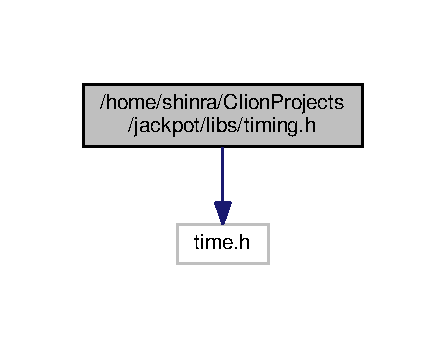
\includegraphics[width=214pt]{timing_8h__incl}
\end{center}
\end{figure}
This graph shows which files directly or indirectly include this file\+:\nopagebreak
\begin{figure}[H]
\begin{center}
\leavevmode
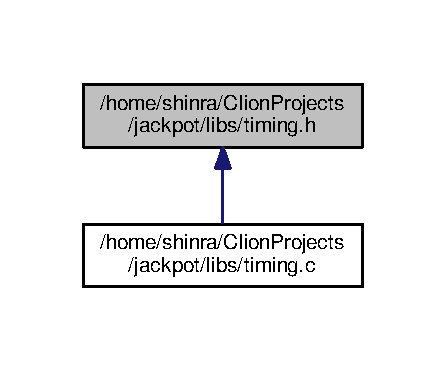
\includegraphics[width=214pt]{timing_8h__dep__incl}
\end{center}
\end{figure}
\subsection*{Functions}
\begin{DoxyCompactItemize}
\item 
void \hyperlink{timing_8h_a606c0b10d8a2b94f79b1d273d2532db0}{start\+Time} ()
\item 
void \hyperlink{timing_8h_af5f394416f4d08f504e88587f60cc489}{stop\+Time} ()
\item 
double \hyperlink{timing_8h_ac56c08903fe71f3197168456aef26524}{get\+Cnt\+Time} ()
\end{DoxyCompactItemize}


\subsection{Detailed Description}
timing's prototypes, allows the user to count the time in secondes, between a start and a stop call. 

\begin{DoxyAuthor}{Author}
B\+U\+F\+F\+O Pierre, D\+A S\+I\+L\+V\+A Gabriel, M\+E\+H\+M\+E\+D Blazevic 
\end{DoxyAuthor}
\begin{DoxyVersion}{Version}
1.\+0 
\end{DoxyVersion}
\begin{DoxyDate}{Date}
25.\+01.\+2017 
\end{DoxyDate}


\subsection{Function Documentation}
\hypertarget{timing_8h_ac56c08903fe71f3197168456aef26524}{\index{timing.\+h@{timing.\+h}!get\+Cnt\+Time@{get\+Cnt\+Time}}
\index{get\+Cnt\+Time@{get\+Cnt\+Time}!timing.\+h@{timing.\+h}}
\subsubsection[{get\+Cnt\+Time}]{\setlength{\rightskip}{0pt plus 5cm}double get\+Cnt\+Time (
\begin{DoxyParamCaption}
{}
\end{DoxyParamCaption}
)}}\label{timing_8h_ac56c08903fe71f3197168456aef26524}
get the difference between the first and the second clock time in seconds \begin{DoxyReturn}{Returns}
elapsed time 
\end{DoxyReturn}
\hypertarget{timing_8h_a606c0b10d8a2b94f79b1d273d2532db0}{\index{timing.\+h@{timing.\+h}!start\+Time@{start\+Time}}
\index{start\+Time@{start\+Time}!timing.\+h@{timing.\+h}}
\subsubsection[{start\+Time}]{\setlength{\rightskip}{0pt plus 5cm}void start\+Time (
\begin{DoxyParamCaption}
{}
\end{DoxyParamCaption}
)}}\label{timing_8h_a606c0b10d8a2b94f79b1d273d2532db0}
get the first clock time \hypertarget{timing_8h_af5f394416f4d08f504e88587f60cc489}{\index{timing.\+h@{timing.\+h}!stop\+Time@{stop\+Time}}
\index{stop\+Time@{stop\+Time}!timing.\+h@{timing.\+h}}
\subsubsection[{stop\+Time}]{\setlength{\rightskip}{0pt plus 5cm}void stop\+Time (
\begin{DoxyParamCaption}
{}
\end{DoxyParamCaption}
)}}\label{timing_8h_af5f394416f4d08f504e88587f60cc489}
get the second clock time 
\hypertarget{wheels_8c}{\section{/home/shinra/\+Clion\+Projects/jackpot/libs/wheels.c File Reference}
\label{wheels_8c}\index{/home/shinra/\+Clion\+Projects/jackpot/libs/wheels.\+c@{/home/shinra/\+Clion\+Projects/jackpot/libs/wheels.\+c}}
}


wheels's functions  


{\ttfamily \#include \char`\"{}wheels.\+h\char`\"{}}\\*
Include dependency graph for wheels.\+c\+:
\nopagebreak
\begin{figure}[H]
\begin{center}
\leavevmode
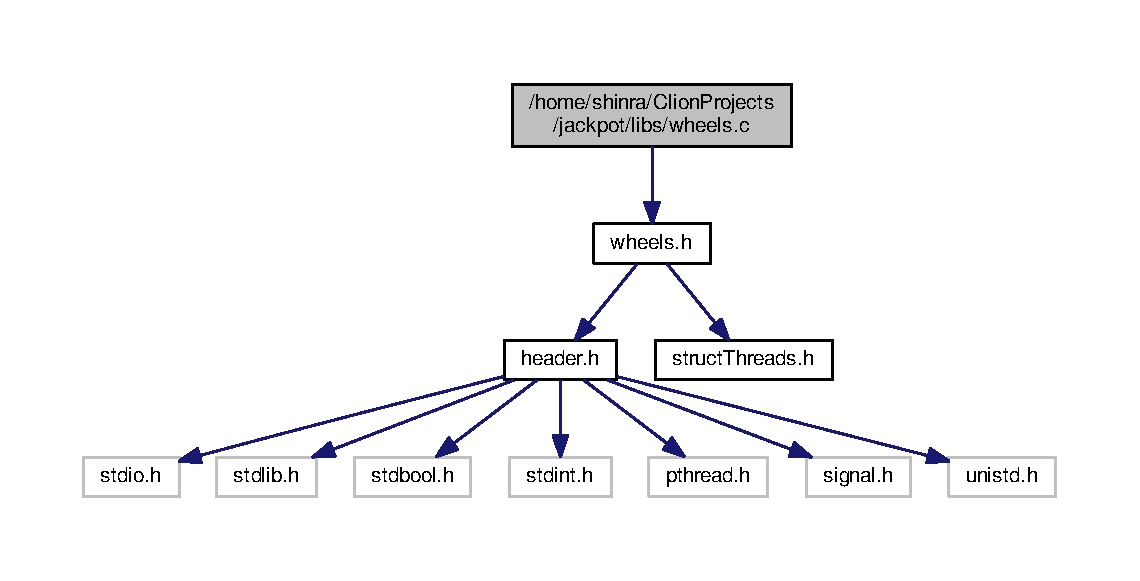
\includegraphics[width=350pt]{wheels_8c__incl}
\end{center}
\end{figure}
\subsection*{Functions}
\begin{DoxyCompactItemize}
\item 
void $\ast$ \hyperlink{wheels_8c_a59ef57831500f5b1144c9e921d61d4a9}{spinner} (void $\ast$thread\+Data)
\item 
double \hyperlink{wheels_8c_a6f17531bb0bf5f5af8f272e54f2b6b25}{wait\+A\+Moment} (struct timespec $\ast$start, struct timespec $\ast$\hyperlink{timing_8c_a94ca335b433152f4af4e062084826ae0}{finish}, int time)
\item 
int \hyperlink{wheels_8c_a325987f64a525993cea919a5060e2933}{Get\+Win} (\hyperlink{structcontroller__t}{controller\+\_\+t} controller\+Data)
\end{DoxyCompactItemize}


\subsection{Detailed Description}
wheels's functions 

\begin{DoxyAuthor}{Author}
B\+U\+F\+F\+O Pierre, D\+A S\+I\+L\+V\+A Gabriel, M\+E\+H\+M\+E\+D Blazevic 
\end{DoxyAuthor}
\begin{DoxyVersion}{Version}
1.\+0 
\end{DoxyVersion}
\begin{DoxyDate}{Date}
25.\+01.\+2017 
\end{DoxyDate}


\subsection{Function Documentation}
\hypertarget{wheels_8c_a325987f64a525993cea919a5060e2933}{\index{wheels.\+c@{wheels.\+c}!Get\+Win@{Get\+Win}}
\index{Get\+Win@{Get\+Win}!wheels.\+c@{wheels.\+c}}
\subsubsection[{Get\+Win}]{\setlength{\rightskip}{0pt plus 5cm}int Get\+Win (
\begin{DoxyParamCaption}
\item[{{\bf controller\+\_\+t}}]{controller\+Data}
\end{DoxyParamCaption}
)}}\label{wheels_8c_a325987f64a525993cea919a5060e2933}
return result of the game 
\begin{DoxyParams}{Parameters}
{\em controller\+Data} & -\/ controller containing the wheels \\
\hline
\end{DoxyParams}
\begin{DoxyReturn}{Returns}
win status, F\+U\+L\+L\+W\+I\+N $\vert$ D\+O\+U\+B\+L\+E\+W\+I\+N $\vert$ L\+O\+S\+T 
\end{DoxyReturn}


Here is the caller graph for this function\+:\nopagebreak
\begin{figure}[H]
\begin{center}
\leavevmode
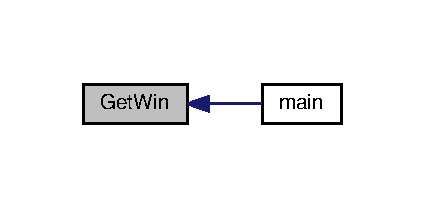
\includegraphics[width=204pt]{wheels_8c_a325987f64a525993cea919a5060e2933_icgraph}
\end{center}
\end{figure}


\hypertarget{wheels_8c_a59ef57831500f5b1144c9e921d61d4a9}{\index{wheels.\+c@{wheels.\+c}!spinner@{spinner}}
\index{spinner@{spinner}!wheels.\+c@{wheels.\+c}}
\subsubsection[{spinner}]{\setlength{\rightskip}{0pt plus 5cm}void$\ast$ spinner (
\begin{DoxyParamCaption}
\item[{void $\ast$}]{thread\+Data}
\end{DoxyParamCaption}
)}}\label{wheels_8c_a59ef57831500f5b1144c9e921d61d4a9}
run the wheels, \char`\"{}rien ne va plus\char`\"{} 
\begin{DoxyParams}{Parameters}
{\em thread\+Data} & -\/ thread's data, containing speed of rotation and current value \\
\hline
\end{DoxyParams}
\begin{DoxyReturn}{Returns}
N\+U\+L\+L 
\end{DoxyReturn}


Here is the call graph for this function\+:\nopagebreak
\begin{figure}[H]
\begin{center}
\leavevmode
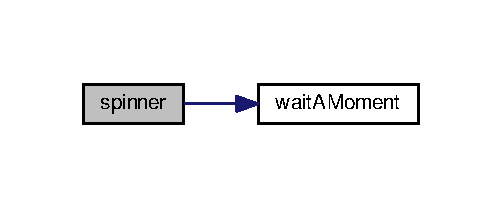
\includegraphics[width=241pt]{wheels_8c_a59ef57831500f5b1144c9e921d61d4a9_cgraph}
\end{center}
\end{figure}




Here is the caller graph for this function\+:\nopagebreak
\begin{figure}[H]
\begin{center}
\leavevmode
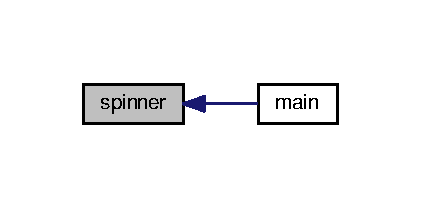
\includegraphics[width=202pt]{wheels_8c_a59ef57831500f5b1144c9e921d61d4a9_icgraph}
\end{center}
\end{figure}


\hypertarget{wheels_8c_a6f17531bb0bf5f5af8f272e54f2b6b25}{\index{wheels.\+c@{wheels.\+c}!wait\+A\+Moment@{wait\+A\+Moment}}
\index{wait\+A\+Moment@{wait\+A\+Moment}!wheels.\+c@{wheels.\+c}}
\subsubsection[{wait\+A\+Moment}]{\setlength{\rightskip}{0pt plus 5cm}double wait\+A\+Moment (
\begin{DoxyParamCaption}
\item[{struct timespec $\ast$}]{start, }
\item[{struct timespec $\ast$}]{finish, }
\item[{int}]{time}
\end{DoxyParamCaption}
)}}\label{wheels_8c_a6f17531bb0bf5f5af8f272e54f2b6b25}
calculate the time to wait before the next refresh with the process time 
\begin{DoxyParams}{Parameters}
{\em start} & -\/ start struct with the timer's begin \\
\hline
{\em finish} & -\/ finish struct with the timer's end \\
\hline
{\em time} & -\/ time in miliseconds to wait \\
\hline
\end{DoxyParams}
\begin{DoxyReturn}{Returns}
time to wait in nanoseconds or 0 if work process too long 
\end{DoxyReturn}


Here is the caller graph for this function\+:\nopagebreak
\begin{figure}[H]
\begin{center}
\leavevmode
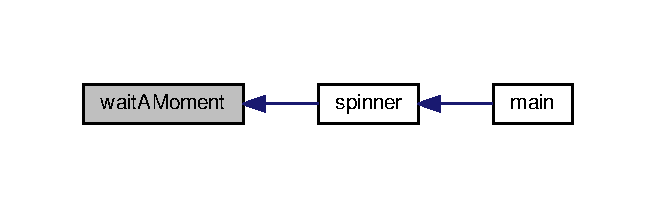
\includegraphics[width=315pt]{wheels_8c_a6f17531bb0bf5f5af8f272e54f2b6b25_icgraph}
\end{center}
\end{figure}



\hypertarget{wheels_8h}{\section{/home/shinra/\+Clion\+Projects/jackpot/libs/wheels.h File Reference}
\label{wheels_8h}\index{/home/shinra/\+Clion\+Projects/jackpot/libs/wheels.\+h@{/home/shinra/\+Clion\+Projects/jackpot/libs/wheels.\+h}}
}


wheels's prototypes  


{\ttfamily \#include \char`\"{}header.\+h\char`\"{}}\\*
{\ttfamily \#include \char`\"{}struct\+Threads.\+h\char`\"{}}\\*
Include dependency graph for wheels.\+h\+:
\nopagebreak
\begin{figure}[H]
\begin{center}
\leavevmode
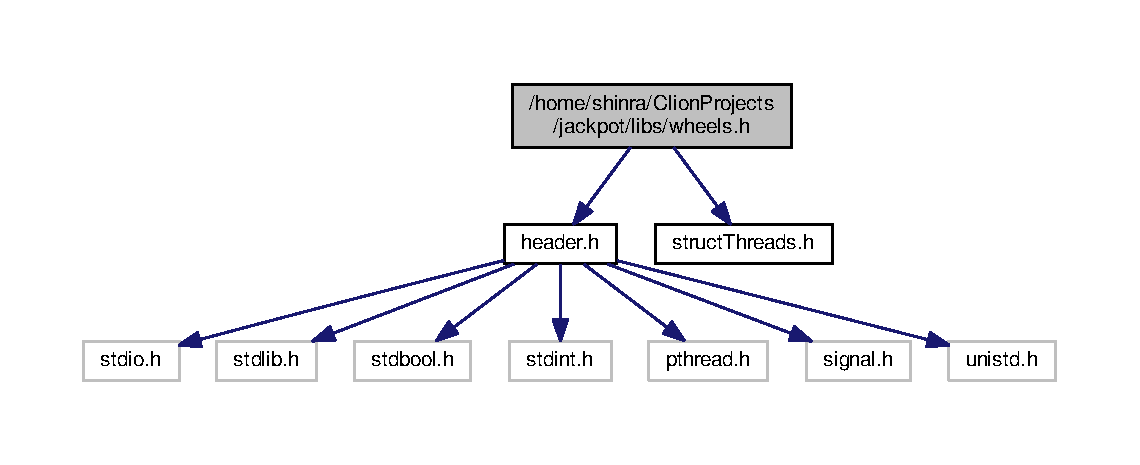
\includegraphics[width=350pt]{wheels_8h__incl}
\end{center}
\end{figure}
This graph shows which files directly or indirectly include this file\+:\nopagebreak
\begin{figure}[H]
\begin{center}
\leavevmode
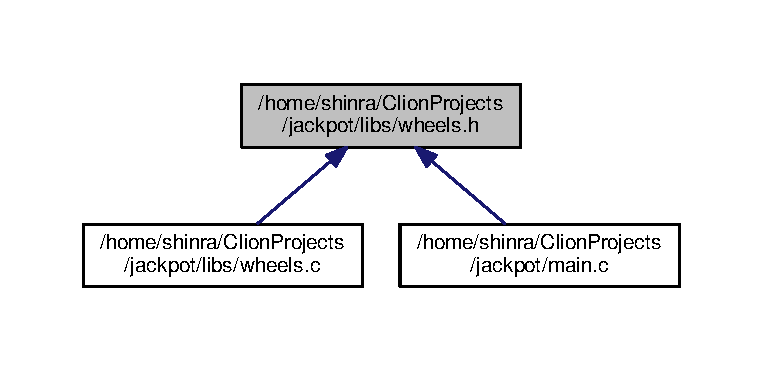
\includegraphics[width=350pt]{wheels_8h__dep__incl}
\end{center}
\end{figure}
\subsection*{Functions}
\begin{DoxyCompactItemize}
\item 
double \hyperlink{wheels_8h_a6f17531bb0bf5f5af8f272e54f2b6b25}{wait\+A\+Moment} (struct timespec $\ast$start, struct timespec $\ast$\hyperlink{timing_8c_a94ca335b433152f4af4e062084826ae0}{finish}, int time)
\item 
void $\ast$ \hyperlink{wheels_8h_a59ef57831500f5b1144c9e921d61d4a9}{spinner} (void $\ast$thread\+Data)
\item 
int \hyperlink{wheels_8h_a325987f64a525993cea919a5060e2933}{Get\+Win} (\hyperlink{structcontroller__t}{controller\+\_\+t} controller\+Data)
\end{DoxyCompactItemize}


\subsection{Detailed Description}
wheels's prototypes 

\begin{DoxyAuthor}{Author}
B\+U\+F\+F\+O Pierre, D\+A S\+I\+L\+V\+A Gabriel, M\+E\+H\+M\+E\+D Blazevic 
\end{DoxyAuthor}
\begin{DoxyVersion}{Version}
1.\+0 
\end{DoxyVersion}
\begin{DoxyDate}{Date}
25.\+01.\+2017 
\end{DoxyDate}


\subsection{Function Documentation}
\hypertarget{wheels_8h_a325987f64a525993cea919a5060e2933}{\index{wheels.\+h@{wheels.\+h}!Get\+Win@{Get\+Win}}
\index{Get\+Win@{Get\+Win}!wheels.\+h@{wheels.\+h}}
\subsubsection[{Get\+Win}]{\setlength{\rightskip}{0pt plus 5cm}int Get\+Win (
\begin{DoxyParamCaption}
\item[{{\bf controller\+\_\+t}}]{controller\+Data}
\end{DoxyParamCaption}
)}}\label{wheels_8h_a325987f64a525993cea919a5060e2933}
return result of the game 
\begin{DoxyParams}{Parameters}
{\em controller\+Data} & -\/ controller containing the wheels \\
\hline
\end{DoxyParams}
\begin{DoxyReturn}{Returns}
win status, F\+U\+L\+L\+W\+I\+N $\vert$ D\+O\+U\+B\+L\+E\+W\+I\+N $\vert$ L\+O\+S\+T 
\end{DoxyReturn}


Here is the caller graph for this function\+:\nopagebreak
\begin{figure}[H]
\begin{center}
\leavevmode
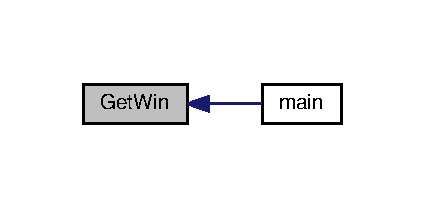
\includegraphics[width=204pt]{wheels_8h_a325987f64a525993cea919a5060e2933_icgraph}
\end{center}
\end{figure}


\hypertarget{wheels_8h_a59ef57831500f5b1144c9e921d61d4a9}{\index{wheels.\+h@{wheels.\+h}!spinner@{spinner}}
\index{spinner@{spinner}!wheels.\+h@{wheels.\+h}}
\subsubsection[{spinner}]{\setlength{\rightskip}{0pt plus 5cm}void$\ast$ spinner (
\begin{DoxyParamCaption}
\item[{void $\ast$}]{thread\+Data}
\end{DoxyParamCaption}
)}}\label{wheels_8h_a59ef57831500f5b1144c9e921d61d4a9}
run the wheels, \char`\"{}rien ne va plus\char`\"{} 
\begin{DoxyParams}{Parameters}
{\em thread\+Data} & -\/ thread's data, containing speed of rotation and current value \\
\hline
\end{DoxyParams}
\begin{DoxyReturn}{Returns}
N\+U\+L\+L 
\end{DoxyReturn}


Here is the call graph for this function\+:\nopagebreak
\begin{figure}[H]
\begin{center}
\leavevmode
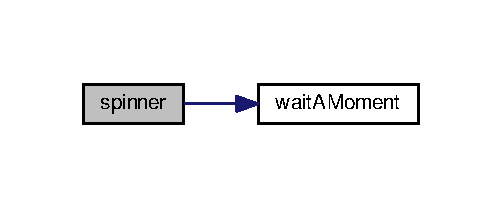
\includegraphics[width=241pt]{wheels_8h_a59ef57831500f5b1144c9e921d61d4a9_cgraph}
\end{center}
\end{figure}




Here is the caller graph for this function\+:\nopagebreak
\begin{figure}[H]
\begin{center}
\leavevmode
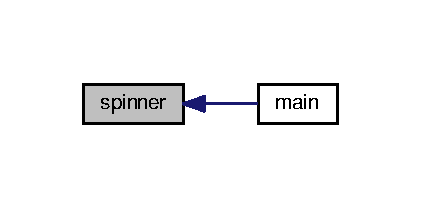
\includegraphics[width=202pt]{wheels_8h_a59ef57831500f5b1144c9e921d61d4a9_icgraph}
\end{center}
\end{figure}


\hypertarget{wheels_8h_a6f17531bb0bf5f5af8f272e54f2b6b25}{\index{wheels.\+h@{wheels.\+h}!wait\+A\+Moment@{wait\+A\+Moment}}
\index{wait\+A\+Moment@{wait\+A\+Moment}!wheels.\+h@{wheels.\+h}}
\subsubsection[{wait\+A\+Moment}]{\setlength{\rightskip}{0pt plus 5cm}double wait\+A\+Moment (
\begin{DoxyParamCaption}
\item[{struct timespec $\ast$}]{start, }
\item[{struct timespec $\ast$}]{finish, }
\item[{int}]{time}
\end{DoxyParamCaption}
)}}\label{wheels_8h_a6f17531bb0bf5f5af8f272e54f2b6b25}
calculate the time to wait before the next refresh with the process time 
\begin{DoxyParams}{Parameters}
{\em start} & -\/ start struct with the timer's begin \\
\hline
{\em finish} & -\/ finish struct with the timer's end \\
\hline
{\em time} & -\/ time in miliseconds to wait \\
\hline
\end{DoxyParams}
\begin{DoxyReturn}{Returns}
time to wait in nanoseconds or 0 if work process too long 
\end{DoxyReturn}


Here is the caller graph for this function\+:\nopagebreak
\begin{figure}[H]
\begin{center}
\leavevmode
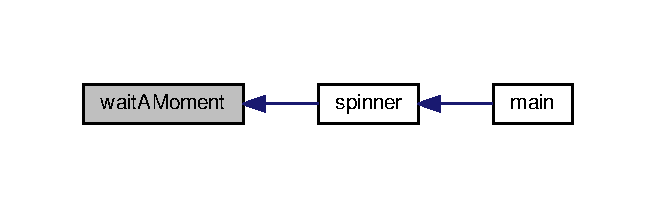
\includegraphics[width=315pt]{wheels_8h_a6f17531bb0bf5f5af8f272e54f2b6b25_icgraph}
\end{center}
\end{figure}



\hypertarget{main_8c}{\section{/home/shinra/\+Clion\+Projects/jackpot/main.c File Reference}
\label{main_8c}\index{/home/shinra/\+Clion\+Projects/jackpot/main.\+c@{/home/shinra/\+Clion\+Projects/jackpot/main.\+c}}
}


programm's entry point  


{\ttfamily \#include $<$math.\+h$>$}\\*
{\ttfamily \#include \char`\"{}libs/header.\+h\char`\"{}}\\*
{\ttfamily \#include \char`\"{}libs/struct\+Threads.\+h\char`\"{}}\\*
{\ttfamily \#include \char`\"{}libs/display.\+h\char`\"{}}\\*
{\ttfamily \#include \char`\"{}libs/wheels.\+h\char`\"{}}\\*
{\ttfamily \#include \char`\"{}libs/signals.\+h\char`\"{}}\\*
Include dependency graph for main.\+c\+:
\nopagebreak
\begin{figure}[H]
\begin{center}
\leavevmode
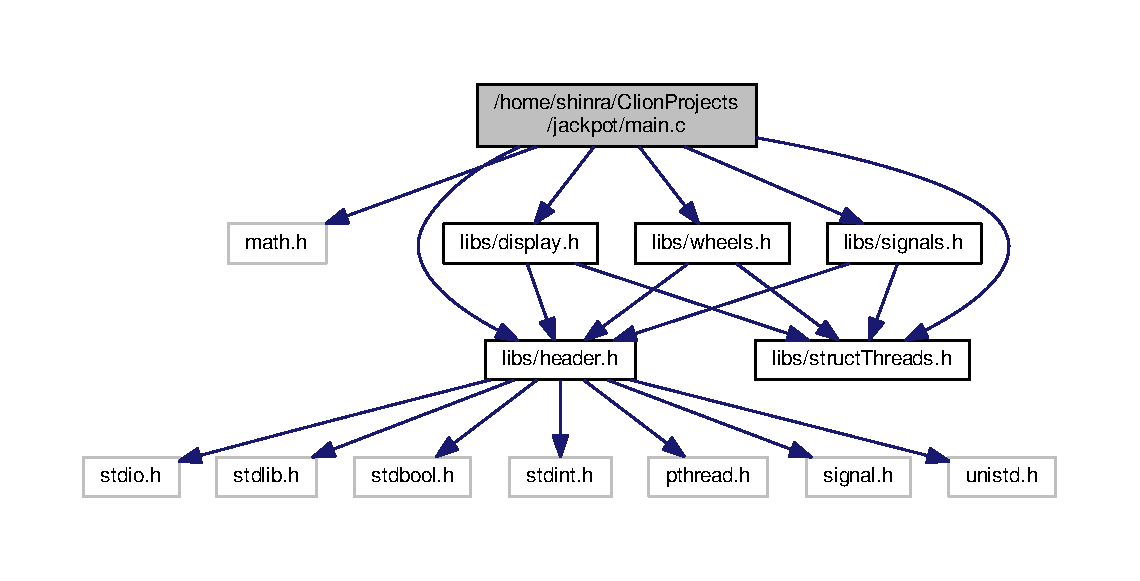
\includegraphics[width=350pt]{main_8c__incl}
\end{center}
\end{figure}
\subsection*{Functions}
\begin{DoxyCompactItemize}
\item 
int \hyperlink{main_8c_a3c04138a5bfe5d72780bb7e82a18e627}{main} (int argc, char $\ast$$\ast$argv)
\end{DoxyCompactItemize}


\subsection{Detailed Description}
programm's entry point 

\begin{DoxyAuthor}{Author}
B\+U\+F\+F\+O Pierre, D\+A S\+I\+L\+V\+A Gabriel, M\+E\+H\+M\+E\+D Blazevic 
\end{DoxyAuthor}
\begin{DoxyVersion}{Version}
1.\+0 
\end{DoxyVersion}
\begin{DoxyDate}{Date}
25.\+01.\+2017 
\end{DoxyDate}


\subsection{Function Documentation}
\hypertarget{main_8c_a3c04138a5bfe5d72780bb7e82a18e627}{\index{main.\+c@{main.\+c}!main@{main}}
\index{main@{main}!main.\+c@{main.\+c}}
\subsubsection[{main}]{\setlength{\rightskip}{0pt plus 5cm}int main (
\begin{DoxyParamCaption}
\item[{int}]{argc, }
\item[{char $\ast$$\ast$}]{argv}
\end{DoxyParamCaption}
)}}\label{main_8c_a3c04138a5bfe5d72780bb7e82a18e627}


Here is the call graph for this function\+:\nopagebreak
\begin{figure}[H]
\begin{center}
\leavevmode
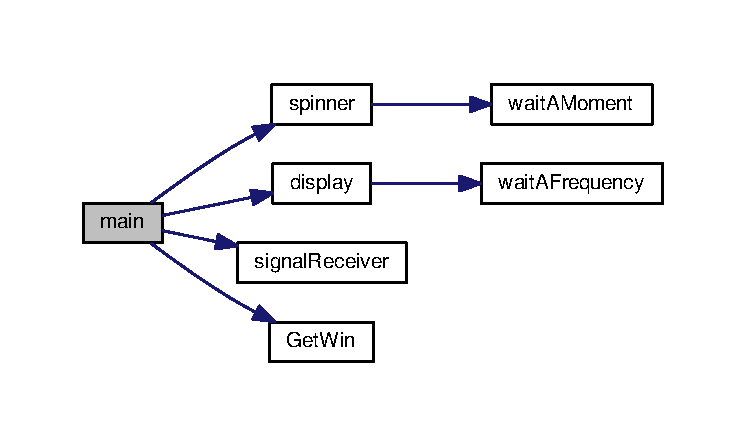
\includegraphics[width=350pt]{main_8c_a3c04138a5bfe5d72780bb7e82a18e627_cgraph}
\end{center}
\end{figure}



%--- End generated contents ---

% Index
\newpage
\phantomsection
\addcontentsline{toc}{chapter}{Index}
\printindex

\end{document}
